%%=============================================================================
%% LaTeX sjabloon voor bachelorproef, HoGent Bedrijf en Organisatie
%% Opleiding Toegepaste Informatica
%%=============================================================================

\documentclass[fleqn,a4paper,12pt]{book}

%%=============================================================================
%% LaTeX sjabloon voor de bachelorproef, HoGent Bedrijf en Organisatie
%% Opleiding toegepaste informatica
%%
%% Structuur en algemene vormgeving. Meestal hoef je hier niets te wijzigen.
%%
%% Vormgeving gebaseerd op "The Legrand Orange Book", version 2.0 (9/2/15)
%% door Mathias Legrand (legrand.mathias@gmail.com) met aanpassingen door
%% Vel (vel@latextemplates.com). Het oorspronkelijke template is te vinden op
%% http://www.LaTeXTemplates.com
%%
%% Aanpassingen voor HoGent toegepaste informatica: 
%%   Bert Van Vreckem <bert.vanvreckem@hogent.be>
%% Licentie: 
%%   CC BY-NC-SA 3.0 (http://creativecommons.org/licenses/by-nc-sa/3.0/)
%%=============================================================================

%%-----------------------------------------------------------------------------
%% Packages
%%-----------------------------------------------------------------------------

\usepackage[top=3cm,bottom=3cm,left=3cm,right=3cm,headsep=10pt,a4paper]{geometry} % Page margins
\usepackage[utf8]{inputenc}  % Accenten gebruiken in tekst (vb. é ipv \'e)
\usepackage{amsfonts}        % AMS math packages: extra wiskundige
\usepackage{amsmath}         %   symbolen (o.a. getallen-
\usepackage{amssymb}         %   verzamelingen N, R, Z, Q, etc.)
\usepackage[english,dutch]{babel}    % Taalinstellingen: woordsplitsingen,
                             %  commando's voor speciale karakters
                             %  ("dutch" voor NL)
\usepackage{iflang}
\usepackage{eurosym}         % Euro-symbool €
\usepackage{geometry}
\usepackage{graphicx}        % Invoegen van tekeningen
\graphicspath{{img/}}       % Specifies the directory where pictures are stored
\usepackage{tikz}            % Required for drawing custom shapes
\usepackage[pdftex,bookmarks=true]{hyperref}
                             % PDF krijgt klikbare links & verwijzingen,
                             %  inhoudstafel
\usepackage{enumitem}        % Customize lists
\setlist{nolistsep}         % Reduce spacing between list items
\usepackage{listings}        % Broncode mooi opmaken
\usepackage{multirow}        % Tekst over verschillende cellen in tabellen
\usepackage{rotating}        % Tabellen en figuren roteren

\usepackage{booktabs}        % Required for nicer horizontal rules in tables

\usepackage{xcolor}          % Required for specifying colors by name
\definecolor{maincolor}{RGB}{0,147,208} % Define the main color used for 
                             % highlighting throughout the book
                             % 0, 147, 208 = officiële kleur HoGent FBO

% Paragraph style: no indent, add space between paragraphs
\setlength{\parindent}{0em}
\setlength{\parskip}{1em}

\usepackage{etoolbox}
\usepackage{titling} % Macros for title, author, etc
\usepackage{lipsum}          % Voor vultekst (lorem ipsum)

%----------------------------------------------------------------------------------------
%	FONTS
%----------------------------------------------------------------------------------------

\usepackage{avant} % Use the Avantgarde font for headings
%\usepackage{times} % Use the Times font for headings
\usepackage{mathptmx} % Use the Adobe Times Roman as the default text font together with math symbols from the Sym­bol, Chancery and Com­puter Modern fonts

\usepackage{microtype} % Slightly tweak font spacing for aesthetics
\usepackage[utf8]{inputenc} % Required for including letters with accents
\usepackage[T1]{fontenc} % Use 8-bit encoding that has 256 glyphs

%------------------------------------------------------------------------------
%	TITLE PAGE
%------------------------------------------------------------------------------

\newcommand{\inserttitlepage}{%
\begin{titlepage}
  \newgeometry{top=2cm,bottom=1.5cm,left=1.5cm,right=1.5cm}
  \begin{center}

    \begingroup
    \rmfamily
    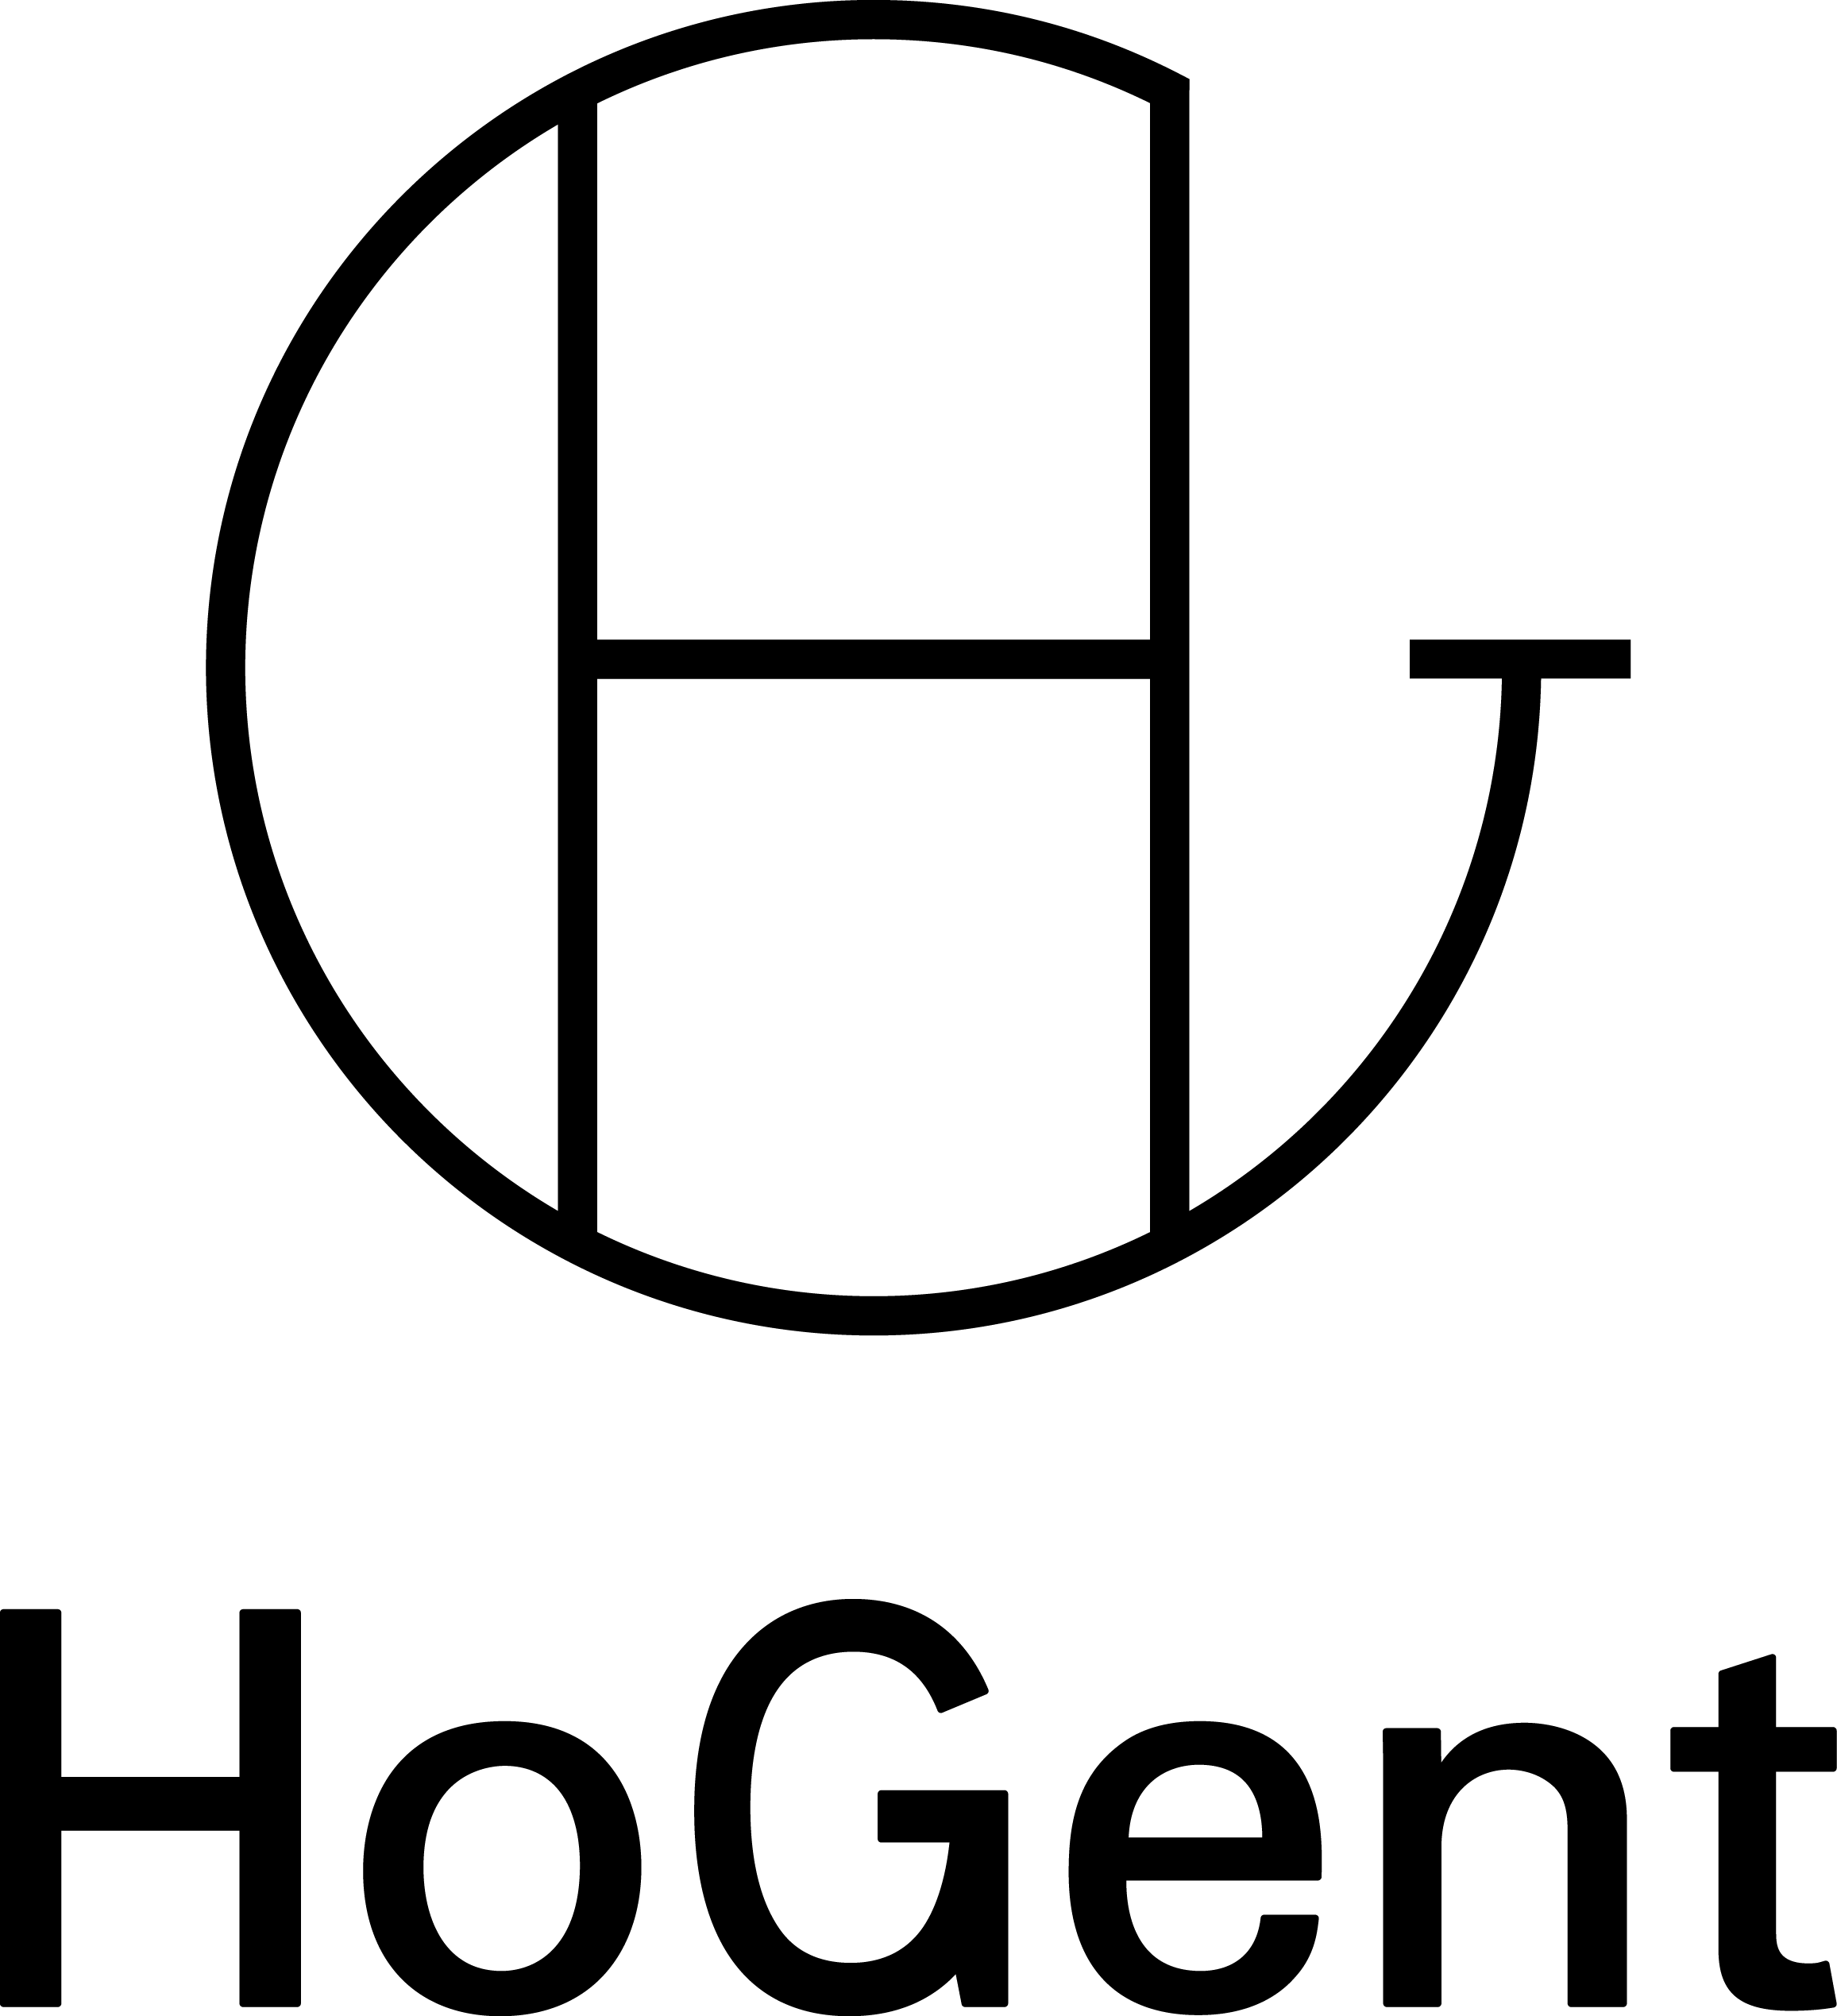
\includegraphics[width=2.5cm]{img/HG-beeldmerk-woordmerk}\\[.5cm]
    Faculteit Bedrijf en Organisatie\\[3cm]
    \titel
    \vfill
    \student\\[3.5cm]
    Scriptie voorgedragen tot het bekomen van de graad van\\professionele bachelor in de toegepaste informatica\\[2cm]
    Promotor:\\
    \promotor\\
    \ifdefempty{\copromotor}{\vspace{2.5cm}}{Co-promotor:\\\copromotor\\[2.5cm]}
    Instelling: \instelling\\[.5cm]
    Academiejaar: \academiejaar\\[.5cm]
    \ifcase \examenperiode \or Eerste \or Tweede \else Derde \fi examenperiode
    \endgroup

  \end{center}
  \restoregeometry
\end{titlepage}
  \emptypage
\begin{titlepage}
  \newgeometry{top=5.35cm,bottom=1.5cm,left=1.5cm,right=1.5cm}
  \begin{center}

    \begingroup
    \rmfamily
    \IfLanguageName{dutch}{Faculteit Bedrijf en Organisatie}{Faculty of Business and Information Management}\\[3cm]
    \titel
    \vfill
    \student\\[3.5cm]
    \IfLanguageName{dutch}{Scriptie voorgedragen tot het bekomen van de graad van\\professionele bachelor in de toegepaste informatica}{Thesis submitted in partial fulfilment of the requirements for the degree of\\professional bachelor of applied computer science}\\[2cm]
    Promotor:\\
    \promotor\\
    \ifdefempty{\copromotor}{\vspace{2.5cm}}{Co-promotor:\\\copromotor\\[2.5cm]}
    \IfLanguageName{dutch}{Instelling}{Institution}: \instelling\\[.5cm]
    \IfLanguageName{dutch}{Academiejaar}{Academic year}: \academiejaar\\[.5cm]
    \IfLanguageName{dutch}{%
    \ifcase \examenperiode \or Eerste \or Tweede \else Derde \fi examenperiode}{%
    \ifcase \examenperiode \or First \or Second \else Third \fi examination period}
    \endgroup

  \end{center}
  \restoregeometry
\end{titlepage}
}

%----------------------------------------------------------------------------------------
%	BIBLIOGRAPHY AND INDEX
%----------------------------------------------------------------------------------------

\usepackage[style=apa,backend=biber]{biblatex}
\usepackage{csquotes}
\DeclareLanguageMapping{dutch}{dutch-apa}
\addbibresource{bachproef-tin.bib} % BibTeX bibliography file
\addbibresource{../voorstel/voorstel.bib}
\defbibheading{bibempty}{}

\usepackage{calc} % For simpler calculation - used for spacing the index letter headings correctly
\usepackage{makeidx} % Required to make an index
\makeindex % Tells LaTeX to create the files required for indexing

%----------------------------------------------------------------------------------------
%	MAIN TABLE OF CONTENTS
%----------------------------------------------------------------------------------------

\usepackage{titletoc} % Required for manipulating the table of contents

\contentsmargin{0cm} % Removes the default margin

% Part text styling
\titlecontents{part}[0cm]
{\addvspace{20pt}\centering\large\bfseries}
{}
{}
{}

% Chapter text styling
\titlecontents{chapter}[1.25cm] % Indentation
{\addvspace{12pt}\large\sffamily\bfseries} % Spacing and font options for chapters
{\color{maincolor!60}\contentslabel[\Large\thecontentslabel]{1.25cm}\color{maincolor}} % Chapter number
{\color{maincolor}}
{\color{maincolor!60}\normalsize\;\titlerule*[.5pc]{.}\;\thecontentspage} % Page number

% Section text styling
\titlecontents{section}[1.25cm] % Indentation
{\addvspace{3pt}\sffamily\bfseries} % Spacing and font options for sections
{\contentslabel[\thecontentslabel]{1.25cm}} % Section number
{}
{\hfill\color{black}\thecontentspage} % Page number
[]

% Subsection text styling
\titlecontents{subsection}[1.25cm] % Indentation
{\addvspace{1pt}\sffamily\small} % Spacing and font options for subsections
{\contentslabel[\thecontentslabel]{1.25cm}} % Subsection number
{}
{\ \titlerule*[.5pc]{.}\;\thecontentspage} % Page number
[]

% List of figures
\titlecontents{figure}[0em]
{\addvspace{-5pt}\sffamily}
{\thecontentslabel\hspace*{1em}}
{}
{\ \titlerule*[.5pc]{.}\;\thecontentspage}
[]

% List of tables
\titlecontents{table}[0em]
{\addvspace{-5pt}\sffamily}
{\thecontentslabel\hspace*{1em}}
{}
{\ \titlerule*[.5pc]{.}\;\thecontentspage}
[]

%----------------------------------------------------------------------------------------
%	MINI TABLE OF CONTENTS IN PART HEADS
%----------------------------------------------------------------------------------------

% Chapter text styling
\titlecontents{lchapter}[0em] % Indenting
{\addvspace{15pt}\large\sffamily\bfseries} % Spacing and font options for chapters
{\color{maincolor}\contentslabel[\Large\thecontentslabel]{1.25cm}\color{maincolor}} % Chapter number
{}
{\color{maincolor}\normalsize\sffamily\bfseries\;\titlerule*[.5pc]{.}\;\thecontentspage} % Page number

% Section text styling
\titlecontents{lsection}[0em] % Indenting
{\sffamily\small} % Spacing and font options for sections
{\contentslabel[\thecontentslabel]{1.25cm}} % Section number
{}
{}

% Subsection text styling
\titlecontents{lsubsection}[.5em] % Indentation
{\normalfont\footnotesize\sffamily} % Font settings
{}
{}
{}

%----------------------------------------------------------------------------------------
%	PAGE HEADERS
%----------------------------------------------------------------------------------------

\usepackage{fancyhdr} % Required for header and footer configuration

\pagestyle{fancy}
\renewcommand{\chaptermark}[1]{\markboth{\sffamily\normalsize\bfseries\chaptername\ \thechapter.\ #1}{}} % Chapter text font settings
\renewcommand{\sectionmark}[1]{\markright{\sffamily\normalsize\thesection\hspace{5pt}#1}{}} % Section text font settings
\fancyhf{} \fancyhead[LE,RO]{\sffamily\normalsize\thepage} % Font setting for the page number in the header
\fancyhead[LO]{\rightmark} % Print the nearest section name on the left side of odd pages
\fancyhead[RE]{\leftmark} % Print the current chapter name on the right side of even pages
\renewcommand{\headrulewidth}{0.5pt} % Width of the rule under the header
\addtolength{\headheight}{2.5pt} % Increase the spacing around the header slightly
\renewcommand{\footrulewidth}{0pt} % Removes the rule in the footer
\fancypagestyle{plain}{\fancyhead{}\renewcommand{\headrulewidth}{0pt}} % Style for when a plain pagestyle is specified

% Removes the header from odd empty pages at the end of chapters
\makeatletter
\renewcommand{\cleardoublepage}{
\clearpage\ifodd\c@page\else
\hbox{}
\vspace*{\fill}
\thispagestyle{empty}
\newpage
\fi}

%----------------------------------------------------------------------------------------
%	THEOREM STYLES
%----------------------------------------------------------------------------------------

\usepackage{amsmath,amsfonts,amssymb,amsthm} % For math equations, theorems, symbols, etc

\newcommand{\intoo}[2]{\mathopen{]}#1\,;#2\mathclose{[}}
\newcommand{\ud}{\mathop{\mathrm{{}d}}\mathopen{}}
\newcommand{\intff}[2]{\mathopen{[}#1\,;#2\mathclose{]}}
\newtheorem{notation}{Notation}[chapter]

% Boxed/framed environments
\newtheoremstyle{maincolornumbox}% % Theorem style name
{0pt}% Space above
{0pt}% Space below
{\normalfont}% % Body font
{}% Indent amount
{\small\bf\sffamily\color{maincolor}}% % Theorem head font
{\;}% Punctuation after theorem head
{0.25em}% Space after theorem head
{\small\sffamily\color{maincolor}\thmname{#1}\nobreakspace\thmnumber{\@ifnotempty{#1}{}\@upn{#2}}% Theorem text (e.g. Theorem 2.1)
\thmnote{\nobreakspace\the\thm@notefont\sffamily\bfseries\color{black}---\nobreakspace#3.}} % Optional theorem note
\renewcommand{\qedsymbol}{$\blacksquare$}% Optional qed square

\newtheoremstyle{blacknumex}% Theorem style name
{5pt}% Space above
{5pt}% Space below
{\normalfont}% Body font
{} % Indent amount
{\small\bf\sffamily}% Theorem head font
{\;}% Punctuation after theorem head
{0.25em}% Space after theorem head
{\small\sffamily{\tiny\ensuremath{\blacksquare}}\nobreakspace\thmname{#1}\nobreakspace\thmnumber{\@ifnotempty{#1}{}\@upn{#2}}% Theorem text (e.g. Theorem 2.1)
\thmnote{\nobreakspace\the\thm@notefont\sffamily\bfseries---\nobreakspace#3.}}% Optional theorem note

\newtheoremstyle{blacknumbox} % Theorem style name
{0pt}% Space above
{0pt}% Space below
{\normalfont}% Body font
{}% Indent amount
{\small\bf\sffamily}% Theorem head font
{\;}% Punctuation after theorem head
{0.25em}% Space after theorem head
{\small\sffamily\thmname{#1}\nobreakspace\thmnumber{\@ifnotempty{#1}{}\@upn{#2}}% Theorem text (e.g. Theorem 2.1)
\thmnote{\nobreakspace\the\thm@notefont\sffamily\bfseries---\nobreakspace#3.}}% Optional theorem note

% Non-boxed/non-framed environments
\newtheoremstyle{maincolornum}% % Theorem style name
{5pt}% Space above
{5pt}% Space below
{\normalfont}% % Body font
{}% Indent amount
{\small\bf\sffamily\color{maincolor}}% % Theorem head font
{\;}% Punctuation after theorem head
{0.25em}% Space after theorem head
{\small\sffamily\color{maincolor}\thmname{#1}\nobreakspace\thmnumber{\@ifnotempty{#1}{}\@upn{#2}}% Theorem text (e.g. Theorem 2.1)
\thmnote{\nobreakspace\the\thm@notefont\sffamily\bfseries\color{black}---\nobreakspace#3.}} % Optional theorem note
\renewcommand{\qedsymbol}{$\blacksquare$}% Optional qed square
\makeatother

% Defines the theorem text style for each type of theorem to one of the three styles above
\newcounter{dummy}
\numberwithin{dummy}{section}
\theoremstyle{maincolornumbox}
\newtheorem{theoremeT}[dummy]{Theorem}
\newtheorem{problem}{Problem}[chapter]
\newtheorem{exerciseT}{Exercise}[chapter]
\theoremstyle{blacknumex}
\newtheorem{exampleT}{Example}[chapter]
\theoremstyle{blacknumbox}
\newtheorem{vocabulary}{Vocabulary}[chapter]
\newtheorem{definitionT}{Definition}[section]
\newtheorem{corollaryT}[dummy]{Corollary}
\theoremstyle{maincolornum}
\newtheorem{proposition}[dummy]{Proposition}

%----------------------------------------------------------------------------------------
%	DEFINITION OF COLORED BOXES
%----------------------------------------------------------------------------------------

\RequirePackage[framemethod=default]{mdframed} % Required for creating the theorem, definition, exercise and corollary boxes

% Theorem box
\newmdenv[skipabove=7pt,
skipbelow=7pt,
backgroundcolor=black!5,
linecolor=maincolor,
innerleftmargin=5pt,
innerrightmargin=5pt,
innertopmargin=5pt,
leftmargin=0cm,
rightmargin=0cm,
innerbottommargin=5pt]{tBox}

% Exercise box
\newmdenv[skipabove=7pt,
skipbelow=7pt,
rightline=false,
leftline=true,
topline=false,
bottomline=false,
backgroundcolor=maincolor!10,
linecolor=maincolor,
innerleftmargin=5pt,
innerrightmargin=5pt,
innertopmargin=5pt,
innerbottommargin=5pt,
leftmargin=0cm,
rightmargin=0cm,
linewidth=4pt]{eBox}

% Definition box
\newmdenv[skipabove=7pt,
skipbelow=7pt,
rightline=false,
leftline=true,
topline=false,
bottomline=false,
linecolor=maincolor,
innerleftmargin=5pt,
innerrightmargin=5pt,
innertopmargin=0pt,
leftmargin=0cm,
rightmargin=0cm,
linewidth=4pt,
innerbottommargin=0pt]{dBox}

% Corollary box
\newmdenv[skipabove=7pt,
skipbelow=7pt,
rightline=false,
leftline=true,
topline=false,
bottomline=false,
linecolor=gray,
backgroundcolor=black!5,
innerleftmargin=5pt,
innerrightmargin=5pt,
innertopmargin=5pt,
leftmargin=0cm,
rightmargin=0cm,
linewidth=4pt,
innerbottommargin=5pt]{cBox}

% Creates an environment for each type of theorem and assigns it a theorem text style from the "Theorem Styles" section above and a colored box from above
\newenvironment{theorem}{\begin{tBox}\begin{theoremeT}}{\end{theoremeT}\end{tBox}}
\newenvironment{exercise}{\begin{eBox}\begin{exerciseT}}{\hfill{\color{maincolor}\tiny\ensuremath{\blacksquare}}\end{exerciseT}\end{eBox}}
\newenvironment{definition}{\begin{dBox}\begin{definitionT}}{\end{definitionT}\end{dBox}}
\newenvironment{example}{\begin{exampleT}}{\hfill{\tiny\ensuremath{\blacksquare}}\end{exampleT}}
\newenvironment{corollary}{\begin{cBox}\begin{corollaryT}}{\end{corollaryT}\end{cBox}}

%----------------------------------------------------------------------------------------
%	REMARK ENVIRONMENT
%----------------------------------------------------------------------------------------

\newenvironment{remark}{\par\vspace{10pt}\small % Vertical white space above the remark and smaller font size
\begin{list}{}{
\leftmargin=35pt % Indentation on the left
\rightmargin=25pt}\item\ignorespaces % Indentation on the right
\makebox[-2.5pt]{\begin{tikzpicture}[overlay]
\node[draw=maincolor!60,line width=1pt,circle,fill=maincolor!25,font=\sffamily\bfseries,inner sep=2pt,outer sep=0pt] at (-15pt,0pt){\textcolor{maincolor}{R}};\end{tikzpicture}} % Orange R in a circle
\advance\baselineskip -1pt}{\end{list}\vskip5pt} % Tighter line spacing and white space after remark

%----------------------------------------------------------------------------------------
%	SECTION NUMBERING IN THE MARGIN
%----------------------------------------------------------------------------------------

\makeatletter
\renewcommand{\@seccntformat}[1]{\llap{\textcolor{maincolor}{\csname the#1\endcsname}\hspace{1em}}}
\renewcommand{\section}{\@startsection{section}{1}{\z@}
{-4ex \@plus -1ex \@minus -.4ex}
{1ex \@plus.2ex }
{\normalfont\large\sffamily\bfseries}}
\renewcommand{\subsection}{\@startsection {subsection}{2}{\z@}
{-3ex \@plus -0.1ex \@minus -.4ex}
{0.5ex \@plus.2ex }
{\normalfont\sffamily\bfseries}}
\renewcommand{\subsubsection}{\@startsection {subsubsection}{3}{\z@}
{-2ex \@plus -0.1ex \@minus -.2ex}
{.2ex \@plus.2ex }
{\normalfont\small\sffamily\bfseries}}
\renewcommand\paragraph{\@startsection{paragraph}{4}{\z@}
{-2ex \@plus-.2ex \@minus .2ex}
{.1ex}
{\normalfont\small\sffamily\bfseries}}

%----------------------------------------------------------------------------------------
%	PART HEADINGS
%----------------------------------------------------------------------------------------

% numbered part in the table of contents
\newcommand{\@mypartnumtocformat}[2]{%
\setlength\fboxsep{0pt}%
\noindent\colorbox{maincolor!20}{\strut\parbox[c][.7cm]{\ecart}{\color{maincolor!70}\Large\sffamily\bfseries\centering#1}}\hskip\esp\colorbox{maincolor!40}{\strut\parbox[c][.7cm]{\linewidth-\ecart-\esp}{\Large\sffamily\centering#2}}}%
%%%%%%%%%%%%%%%%%%%%%%%%%%%%%%%%%%
% unnumbered part in the table of contents
\newcommand{\@myparttocformat}[1]{%
\setlength\fboxsep{0pt}%
\noindent\colorbox{maincolor!40}{\strut\parbox[c][.7cm]{\linewidth}{\Large\sffamily\centering#1}}}%
%%%%%%%%%%%%%%%%%%%%%%%%%%%%%%%%%%
\newlength\esp
\setlength\esp{4pt}
\newlength\ecart
\setlength\ecart{1.2cm-\esp}
\newcommand{\thepartimage}{}%
\newcommand{\partimage}[1]{\renewcommand{\thepartimage}{#1}}%
\def\@part[#1]#2{%
\ifnum \c@secnumdepth >-2\relax%
\refstepcounter{part}%
\addcontentsline{toc}{part}{\texorpdfstring{\protect\@mypartnumtocformat{\thepart}{#1}}{\partname~\thepart\ ---\ #1}}
\else%
\addcontentsline{toc}{part}{\texorpdfstring{\protect\@myparttocformat{#1}}{#1}}%
\fi%
\startcontents%
\markboth{}{}%
{\thispagestyle{empty}%
\begin{tikzpicture}[remember picture,overlay]%
\node at (current page.north west){\begin{tikzpicture}[remember picture,overlay]%
\fill[maincolor!20](0cm,0cm) rectangle (\paperwidth,-\paperheight);
\node[anchor=north] at (4cm,-3.25cm){\color{maincolor!40}\fontsize{220}{100}\sffamily\bfseries\@Roman\c@part};
\node[anchor=south east] at (\paperwidth-1cm,-\paperheight+1cm){\parbox[t][][t]{8.5cm}{
\printcontents{l}{0}{\setcounter{tocdepth}{1}}%
}};
\node[anchor=north east] at (\paperwidth-1.5cm,-3.25cm){\parbox[t][][t]{15cm}{\strut\raggedleft\color{white}\fontsize{30}{30}\sffamily\bfseries#2}};
\end{tikzpicture}};
\end{tikzpicture}}%
\@endpart}
\def\@spart#1{%
\startcontents%
\phantomsection
{\thispagestyle{empty}%
\begin{tikzpicture}[remember picture,overlay]%
\node at (current page.north west){\begin{tikzpicture}[remember picture,overlay]%
\fill[maincolor!20](0cm,0cm) rectangle (\paperwidth,-\paperheight);
\node[anchor=north east] at (\paperwidth-1.5cm,-3.25cm){\parbox[t][][t]{15cm}{\strut\raggedleft\color{white}\fontsize{30}{30}\sffamily\bfseries#1}};
\end{tikzpicture}};
\end{tikzpicture}}
\addcontentsline{toc}{part}{\texorpdfstring{%
\setlength\fboxsep{0pt}%
\noindent\protect\colorbox{maincolor!40}{\strut\protect\parbox[c][.7cm]{\linewidth}{\Large\sffamily\protect\centering #1\quad\mbox{}}}}{#1}}%
\@endpart}
\def\@endpart{\vfil\newpage
\if@twoside
\if@openright
\null
\thispagestyle{empty}%
\newpage
\fi
\fi
\if@tempswa
\twocolumn
\fi}

%----------------------------------------------------------------------------------------
%	CHAPTER HEADINGS
%----------------------------------------------------------------------------------------

% A switch to conditionally include a picture, implemented by  Christian Hupfer
\newif\ifusechapterimage
\usechapterimagetrue
\newcommand{\thechapterimage}{}%
\newcommand{\chapterimage}[1]{\ifusechapterimage\renewcommand{\thechapterimage}{#1}\fi}%
\def\@makechapterhead#1{%
{\parindent \z@ \raggedright \normalfont
\ifnum \c@secnumdepth >\m@ne
\if@mainmatter
\begin{tikzpicture}[remember picture,overlay]
\node at (current page.north west)
{\begin{tikzpicture}[remember picture,overlay]
\node[anchor=north west,inner sep=0pt] at (0,0) {\ifusechapterimage\includegraphics[width=\paperwidth]{\thechapterimage}\fi};
\draw[anchor=west] (\Gm@lmargin,-9cm) node [line width=2pt,rounded corners=15pt,draw=maincolor,fill=white,fill opacity=0.5,inner sep=15pt]{\strut\makebox[22cm]{}};
\draw[anchor=west] (\Gm@lmargin+.3cm,-9cm) node {\huge\sffamily\bfseries\color{black}\thechapter. #1\strut};
\end{tikzpicture}};
\end{tikzpicture}
\else
\begin{tikzpicture}[remember picture,overlay]
\node at (current page.north west)
{\begin{tikzpicture}[remember picture,overlay]
\node[anchor=north west,inner sep=0pt] at (0,0) {\ifusechapterimage\includegraphics[width=\paperwidth]{\thechapterimage}\fi};
\draw[anchor=west] (\Gm@lmargin,-9cm) node [line width=2pt,rounded corners=15pt,draw=maincolor,fill=white,fill opacity=0.5,inner sep=15pt]{\strut\makebox[22cm]{}};
\draw[anchor=west] (\Gm@lmargin+.3cm,-9cm) node {\huge\sffamily\bfseries\color{black}#1\strut};
\end{tikzpicture}};
\end{tikzpicture}
\fi\fi\par\vspace*{270\p@}}}

%-------------------------------------------

\def\@makeschapterhead#1{%
\begin{tikzpicture}[remember picture,overlay]
\node at (current page.north west)
{\begin{tikzpicture}[remember picture,overlay]
\node[anchor=north west,inner sep=0pt] at (0,0) {\ifusechapterimage\includegraphics[width=\paperwidth]{\thechapterimage}\fi};
\draw[anchor=west] (\Gm@lmargin,-9cm) node [line width=2pt,rounded corners=15pt,draw=maincolor,fill=white,fill opacity=0.5,inner sep=15pt]{\strut\makebox[22cm]{}};
\draw[anchor=west] (\Gm@lmargin+.3cm,-9cm) node {\huge\sffamily\bfseries\color{black}#1\strut};
\end{tikzpicture}};
\end{tikzpicture}
\par\vspace*{270\p@}}
\makeatother

%----------------------------------------------------------------------------------------
%	HYPERLINKS IN THE DOCUMENTS
%----------------------------------------------------------------------------------------

\usepackage{hyperref}
\hypersetup{hidelinks,backref=true,pagebackref=true,hyperindex=true,colorlinks=false,breaklinks=true,urlcolor= maincolor,bookmarks=true,bookmarksopen=false,pdftitle={Title},pdfauthor={Author}}
\usepackage{bookmark}
\bookmarksetup{
open,
numbered,
addtohook={%
\ifnum\bookmarkget{level}=0 % chapter
\bookmarksetup{bold}%
\fi
\ifnum\bookmarkget{level}=-1 % part
\bookmarksetup{color=maincolor,bold}%
\fi
}
}

%----------------------------------------------------------------------------------------
%	Java source code
%----------------------------------------------------------------------------------------

% Commando voor invoegen Java-broncodebestanden (dank aan Niels Corneille)
% Gebruik:
%   \codefragment{source/MijnKlasse.java}{Uitleg bij de code}
%
% Je kan dit aanpassen aan de taal die je zelf het meeste gebruikt in je
% bachelorproef.
\newcommand{\codefragment}[2]{ \lstset{%
  language=java,
  breaklines=true,
  float=th,
  caption={#2},
  basicstyle=\scriptsize,
  frame=single,
  extendedchars=\true
}
\lstinputlisting{#1}}

% Leeg blad
\newcommand{\emptypage}{%
\newpage
\thispagestyle{empty}
\mbox{}
\newpage
}


%%---------- Documenteigenschappen --------------------------------------------
%% TODO: Vul dit aan met je eigen info:

% Je eigen naam
\newcommand{\student}{Hu Ocean Li}

% De naam van je promotor (lector van de opleiding)
\newcommand{\promotor}{Olivier Rosseel}

% De naam van je co-promotor. Als je promotor ook je opdrachtgever is en je
% dus ook inhoudelijk begeleidt (en enkel dan!), mag je dit leeg laten.
\newcommand{\copromotor}{}

% Indien je bachelorproef in opdracht van/in samenwerking met een bedrijf of
% externe organisatie geschreven is, geef je hier de naam. Zoniet laat je dit
% zoals het is.
\newcommand{\instelling}{Hogent  Faculteit Bedrijf en Organisatie}

% De titel van het rapport/bachelorproef
\newcommand{\titel}{Een Blockchain-gebaseerd stemsysteem, analyse en praktische gids voor het opzetten}

% Datum van indienen (gebruik telkens de deadline, ook al geef je eerder af)
\newcommand{\datum}{27 mei 2016}

% Academiejaar
\newcommand{\academiejaar}{2015-2016}

% Examenperiode
%  - 1e semester = 1e examenperiode => 1
%  - 2e semester = 2e examenperiode => 2
%  - tweede zit  = 3e examenperiode => 3
\newcommand{\examenperiode}{2}

%%=============================================================================
%% Inhoud document
%%=============================================================================
\usepackage{amsmath}
\usepackage{nccmath}
\usepackage{graphicx}
\usepackage{listings}
\usepackage{color}
\definecolor{lightgray}{rgb}{.9,.9,.9}
\definecolor{darkgray}{rgb}{.4,.4,.4}
\definecolor{purple}{rgb}{0.65, 0.12, 0.82}
\definecolor{ao(english)}{rgb}{0.0, 0.5, 0.0}
\lstdefinelanguage{JavaScriptSolidity}{
	keywords={pragma,uint,struct,string,break, case, catch, continue, memory, debugger, default, delete, do, else, false, finally, for, function, if, in, instanceof, new, null, return, constructor, contract, switch, this, constructor, throw, true, try, typeof, it, assert, mapping, var, void, while, with, public, private},
	morecomment=[l]{//},
	morecomment=[s]{/*}{*/},
	morestring=[b]',
	morestring=[b]",
	ndkeywords={ class, Election, Candidate, electionInstance, export, boolean, throw, implements, import, this},
	keywordstyle=\color{blue}\bfseries,
	ndkeywordstyle=\color{ao(english)}\bfseries,
	identifierstyle=\color{black},
	commentstyle=\color{darkgray}\ttfamily,
	stringstyle=\color{orange}\ttfamily,
	sensitive=true
}

\lstset{
	language=JavaScriptSolidity,
	extendedchars=true,
	basicstyle=\footnotesize\ttfamily,
	showstringspaces=false,
	showspaces=false,
	numbers=left,
	numberstyle=\footnotesize,
	numbersep=9pt,
	tabsize=2,
	breaklines=true,
	showtabs=false,
	captionpos=b
}


\begin{document}

%---------- Taalselectie ------------------------------------------------------
% Als je je bachelorproef in het Engels schrijft, haal dan onderstaande regel
% uit commentaar. Let op: de tekst op de voorkaft blijft in het Nederlands, en
% dat is ook de bedoeling!

%\selectlanguage{english}

%---------- Titelblad ---------------------------------------------------------
\inserttitlepage

%---------- Samenvatting, voorwoord -------------------------------------------
\usechapterimagefalse
%%=============================================================================
%% Voorwoord
%%=============================================================================

\chapter*{Woord vooraf}
\label{ch:voorwoord}

%% TODO:
%% Het voorwoord is het enige deel van de bachelorproef waar je vanuit je
%% eigen standpunt (``ik-vorm'') mag schrijven. Je kan hier bv. motiveren
%% waarom jij het onderwerp wil bespreken.
%% Vergeet ook niet te bedanken wie je geholpen/gesteund/... heeft

Ter voltooiing van mijn opleiding als Bachelor in de toegepaste informatica presenteer ik u deze scriptie.  Voor ik aan deze bachelorproef begon had ik slechts een flauwe notie van wat blockchain was. Het idee om blockchain-gebaseerde stemsystemen te onderzoeken ontstond dan ook uit pure interesse, na verscheidene interessante artikels te hebben gelezen. Ik werd dus in een wereld geworpen waar ik aanvankelijk weinig van begreep, geleidelijk aan slaagde ik er gelukkig in om kennis rond het onderwerp op te bouwen. Gedurende dit onderzoek leerde ik enorm veel bij, zodat ik mijzelf nu een blockchain-developer kan noemen.

De voltooiing van dit onderzoek vormt voor mij  de afsluiting van de voorbije drie jaar op de Hogeschool Gent, een periode waarin ik mijn technische kennis beetje bij beetje zag groeien leerde om mijzelf steeds te blijven bijscholen, vooral die laatste vaardigheid kwam erg van pas tijdens dit onderzoek en het is daarvoor dat ik alle leerkrachten en medewerkers van mijn opleiding zou willen bedanken.

Mijn dank gaat specifiek ook uit naar mijn promotor, Olivier Rosseel, wiens praktische tips en suggesties bijzonder waardevol waren, net als de literatuur die hij mij  heeft aangereikt.

Verder zou ik ook mijn co-promotor willen bedanken, niet alleen voor het lezen van mijn bachelorproef, maar ook voor het inspireren ervan. Zijn artikel over blockchain-gebaseerd stemmen was een van de redenen die mij aanzette tot het voeren van dit onderzoek.

Als laatste zou ik ook mijn familie en vriendin willen bedanken, niet alleen voor het nalezen en verbeteren van deze scriptie, maar ook voor alle steun die ze mij steeds boden en omdat ik steeds op hen kan rekenen.








%%=============================================================================
%% Samenvatting
%%=============================================================================

% TODO: De "abstract" of samenvatting is een kernachtige (~ 1 blz. voor een
% thesis) synthese van het document.
%
% Deze aspecten moeten zeker aan bod komen:
% - Context: waarom is dit werk belangrijk?
% - Nood: waarom moest dit onderzocht worden?
% - Taak: wat heb je precies gedaan?
% - Object: wat staat in dit document geschreven?
% - Resultaat: wat was het resultaat?
% - Conclusie: wat is/zijn de belangrijkste conclusie(s)?
% - Perspectief: blijven er nog vragen open die in de toekomst nog kunnen
%    onderzocht worden? Wat is een mogelijk vervolg voor jouw onderzoek?
%
% LET OP! Een samenvatting is GEEN voorwoord!

%%---------- Nederlandse samenvatting -----------------------------------------
%
% TODO: Als je je bachelorproef in het Engels schrijft, moet je eerst een
% Nederlandse samenvatting invoegen. Haal daarvoor onderstaande code uit
% commentaar.
% Wie zijn bachelorproef in het Nederlands schrijft, kan dit negeren, de inhoud
% wordt niet in het document ingevoegd.

\IfLanguageName{english}{%
\selectlanguage{dutch}
\chapter*{Samenvatting}
\lipsum[1-4]
\selectlanguage{english}
}{}

%%---------- Samenvatting -----------------------------------------------------
% De samenvatting in de hoofdtaal van het document

\chapter*{\IfLanguageName{dutch}{Samenvatting}{Abstract}}

\lipsum[1-4]


%---------- Inhoudstafel ------------------------------------------------------
\pagestyle{empty} % No headers
\tableofcontents % Print the table of contents itself
\cleardoublepage % Forces the first chapter to start on an odd page so it's on the right
\pagestyle{fancy} % Print headers again

%---------- Lijst figuren, afkortingen, ... -----------------------------------

% Indien gewenst kan je hier een lijst van figuren/tabellen opgeven. Geef in
% dat geval je figuren/tabellen altijd een korte beschrijving:
%
%  \caption[korte beschrijving]{uitgebreide beschrijving}

\listoffigures
\listoftables

% Als je een lijst van afkortingen of termen wil toevoegen, dan hoort die
% hier thuis. Gebruik bijvoorbeeld de ``glossaries' package.
% https://www.sharelatex.com/learn/Glossaries

%%---------- Kern -------------------------------------------------------------

%%=============================================================================
%% Inleiding
%%=============================================================================

\chapter{Inleiding}
\label{ch:inleiding}

%%De inleiding moet de lezer net genoeg informatie verschaffen om het onderwerp te begrijpen en in te zien waarom de onderzoeksvraag de moeite waard is om te onderzoeken. In de inleiding ga je literatuurverwijzingen beperken, zodat de tekst vlot leesbaar blijft. Je kan de inleiding verder onderverdelen in secties als dit de tekst verduidelijkt. Zaken die aan bod kunnen komen in de inleiding~\autocite{Pollefliet2011}:

Democratisch stemmen is een cruciaal beslissingsmechanisme  dat aanwezig is in iedere laag van onze moderne samenleving. Het vormt  de basis van het politieke systeem in veel landen en ook de bedrijfswereld is er van doordrongen. Stemprocessen zijn niet meer weg te denken uit de organisaties van vandaag: of het nu gaat over kleine besluiten op het allerlaagste niveau of over grote strategische beslissingen op het allerhoogste, de verantwoordelijkheid voor het maken van keuzes is bijna altijd beter besteed aan een groep met diverse visies en talenten dan aan één enkele persoon. Het totale belang van alle beslissingen die worden bekomen uit stemmen is niet te onderschatten, het is gigantisch. Dit is het belang van het stemproces.

De volgende vraag dringt zich echter op: hoe houdt men een iets waar zoveel van afhangt betrouwbaar, veilig en eerlijk? In de meeste gevallen blijkt het antwoord op die vraag vrij eenvoudig: waar het aantal participanten klein is, kan het resultaat van de stemming gemakkelijk door iedere deelnemer of observator geverifieerd worden. Iedereen kan getuigen dat alles correct verloopt en dat maakt de kans op frauduleuze praktijken veel kleiner. Wordt het aantal participanten echter groter, dan is een dergelijk systeem onmogelijk. In zo'n geval bepaalt men het resultaat van de stemming via een \textit{centrale autoriteit}. Deze derde partij voert een controlerende functie uit en garandeert de betrouwbaarheid voor alle participanten. Bij nationale verkiezingen is dit bijvoorbeeld het stembureau. 
\newpage
\section{Probleemstelling}
\label{sec:probleemstelling}
Er zijn verschillende problemen bij het gebruik van een centrale autoriteit. Eén daarvan is dat het volledige systeem gebaseerd is op vertrouwen. De kiezer brengt een stem uit en de centrale autoriteit doet de rest. Men heeft weinig\footnote{In sommige landen, waaronder Nederland, kan de kiezer de telling van stemmen bijwonen.} tot geen inzicht in het verdere proces. Er is geen manier om te controleren of de eigen stem werd meegeteld, om zich van de correctheid van het eindresultaat te verzekeren. Eén van de gevaren is dus het risico op machtsmisbruik vanuit de centrale autoriteit. Voorafbepaalde en frauduleuze verkiezingen komen op die manier nog veel te vaak voor in ontwikkelingslanden. Dit gebrek aan transparantie is niet alleen gevaarlijk, het is ook fundamenteel ondemocratisch.

Eigenlijk vertrouwen we bijna blindelings op de goede wil en correctheid van de centrale autoriteit, terwijl daar geen goede reden voor is, in tegendeel zelfs. Ook een goedwillige centrale autoriteit kan fouten maken. Al worden er vaak controles gebruikt, toch zijn zowel menselijke als technische fouten op termijn onvermijdelijk. Een persoon die handmatig stemmen telt kan bijvoorbeeld af en toe fouten maken, zelfs een elektronische stemmachine laat het wel eens afweten. Naast top-down electorale fraude en onopzettelijke fouten zijn er ook nieuwe bedreigingen voor de correctheid en eerlijkheid van verkiezingen. Door de digitalisering van het stemproces worden fenomenen zoals hacking, cyberaanvallen en identiteitsdiefstal ook potentiële gevaren. Externe partijen kunnen proberen in een verkiezing te frauderen, waarbij de elektronische centrale meestal het mikpunt vormt. Toch zien we in dat veel landen in toenemende mate gebruik maken van elektronische systemen in hun verkiezingen.

Een potentiële oplossing biedt zich aan in de vorm van blockchain. Deze datastructuur werd in feite net voor dit soort problemen ontwikkeld. De oorsprong van blockchain is gelinkt aan de eerste gedecentraliseerde digitale munteenheid:  Bitcoin. Net als bij het stemproces, wordt de legitimiteit van de klassieke munteenheden bepaald door hun centrale autoriteit, de centrale banken. De structuur die we vandaag kennen als blockchain zorgt ervoor dat Bitcoin geen centrale bank nodig heeft. Met een hypothetisch blockchain gebaseerd stemsysteem willen we dus het volgende bereiken: een stemsysteem waarin we niet meer hoeven te vertrouwen op een stembureau of andere vorm van centrale autoriteit, maar waarin iedere kiezer de verkiezingsresultaten voor zichzelf kan verifiëren.

Onderzoek naar de mogelijkheden van blockchain stemmen is zeker de moeite waard. Specifiek kan deze scriptie een grote meerwaarde bieden voor ontwikkelaars die interesse hebben in het implementeren van een stemsysteem. De aangeboden handleiding kan hen daarbij op weg helpen. Daarnaast kan ook iedereen die geïnteresseerd is in zaken als burgerparticipatie, verkiezingen en democratie, waaronder co-promotor Dr. Jurgen Goossens, meerwaarde in de scriptie vinden. Deze is - op de handleiding na - gestructureerd en geschreven om perspectief te verschaffen in de complexe aard van blockchain.
\section{Onderzoeksvraag}
\label{sec:onderzoeksvraag}
\begin{itemize}
	\item Wat zijn de voor- en nadelen van blockchain-technologie in het kader van een stemsysteem?
	\item Is er sprake van een onoverkomelijk schaalbaarheidsprobleem voor blockchain-technologie?
	\item Welke tools heeft men nodig om een blockchain-gebaseerd stemsysteem op te zetten en wat zijn de voor- en nadelen hiervan?
	\item Is een blockchain-gebaseerd stemsysteem haalbaar in de praktijk?
\end{itemize}
\section{Onderzoeksdoelstelling}
\label{sec:onderzoeksdoelstelling}
Het beoogde resultaat van deze scriptie is drievoudig:

Ten eerste wenst dit onderzoek een zo helder mogelijk antwoord te bieden op de onderzoeksvragen (\ref{sec:onderzoeksvraag}). We kijken naar de technologie en de implementaties van vandaag om te ontdekken wat de toekomst zal bieden.

Ten tweede wenst dit onderzoek zelf een kleinschalig blockchain gebaseerd stemsysteem te ontwikkelen. Succescriteria zijn dat het systeem \textit{betrouwbaarder}, \textit{efficiënter} en \textit{ten minste even schaalbaar} is als de huidige gecentraliseerde methode. Het ontwikkelen van een grootschalig systeem dat aan deze voorwaarden voldoet valt buiten de scope van deze bachelorproef.

Ten derde wenst dit onderzoek ook een handleiding te bieden waarin de ontwikkeling van het blockchain-gebaseerd stemsysteem stap voor stap wordt toegelicht. Deze handleiding moet software-ontwikkelaars met interesse  in het onderwerp aan de slag kunnen helpen.
\section{Opzet van deze bachelorproef}
\label{sec:opzet-bachelorproef}
% Het is gebruikelijk aan het einde van de inleiding een overzicht te
% geven van de opbouw van de rest van de tekst. Deze sectie bevat al een aanzet
% die je kan aanvullen/aanpassen in functie van je eigen tekst.
De rest van deze bachelorproef is als volgt opgebouwd:

In Hoofdstuk~\ref{ch:stand-van-zaken} wordt een overzicht gegeven van de stand van zaken binnen het onderzoeksdomein, op basis van een literatuurstudie.

In Hoofdstuk~\ref{ch:methodologie} wordt de methodologie toegelicht en worden de gebruikte onderzoekstechnieken besproken om een antwoord te kunnen formuleren op de onderzoeksvragen.

In Hoofdstuk~\ref{ch:handleiding} wordt de handleiding gegeven om een eigen implementatie van een blockchain-gebaseerd stemsysteem te realiseren.

In Hoofdstuk~\ref{ch:conclusie}, tenslotte, wordt de conclusie gegeven en een antwoord geformuleerd op de onderzoeksvragen. Daarbij wordt ook een aanzet gegeven voor toekomstig onderzoek binnen dit domein.
\chapter{Stand van zaken}
\label{ch:stand-van-zaken}

% Tip: Begin elk hoofdstuk met een paragraaf inleiding die beschrijft hoe
% dit hoofdstuk past binnen het geheel van de bachelorproef. Geef in het
% bijzonder aan wat de link is met het vorige en volgende hoofdstuk.

% Pas na deze inleidende paragraaf komt de eerste sectiehoofding.

Dit hoofdstuk bevat je literatuurstudie. De inhoud gaat verder op de inleiding, maar zal het onderwerp van de bachelorproef *diepgaand* uitspitten. De bedoeling is dat de lezer na lezing van dit hoofdstuk helemaal op de hoogte is van de huidige stand van zaken (state-of-the-art) in het onderzoeksdomein. Iemand die niet vertrouwd is met het onderwerp, weet er nu voldoende om de rest van het verhaal te kunnen volgen, zonder dat die er nog andere informatie moet over opzoeken \autocite{Pollefliet2011}.

Je verwijst bij elke bewering die je doet, vakterm die je introduceert, enz. naar je bronnen. In \LaTeX{} kan dat met het commando \texttt{$\backslash${textcite\{\}}} of \texttt{$\backslash${autocite\{\}}}. Als argument van het commando geef je de ``sleutel'' van een ``record'' in een bibliografische databank in het Bib\TeX{}-formaat (een tekstbestand). Als je expliciet naar de auteur verwijst in de zin, gebruik je \texttt{$\backslash${}textcite\{\}}.
Soms wil je de auteur niet expliciet vernoemen, dan gebruik je \texttt{$\backslash${}autocite\{\}}. In de volgende paragraaf een voorbeeld van elk.

\textcite{Knuth1998} schreef een van de standaardwerken over sorteer- en zoekalgoritmen. Experten zijn het erover eens dat cloud computing een interessante opportuniteit vormen, zowel voor gebruikers als voor dienstverleners op vlak van informatietechnologie~\autocite{Creeger2009}.
\newpage
\section{Blockchain}
\label{sec:blockchain}
	\subsection*{Inleiding}
	In de eerste deel van dit hoofstuk wordt  Blockchain besproken. We introduceren een basis-idee van wat een blockchain is. We doen dit aan de hand van een paper dat aan de wereld geintroduceert werd in 2008. In Bitcoin: A Peer-to-Peer Electronic Cash System beschrijft een auteur, onder het pseudoniem Satoshi Nakamoto voor het eerst een monetair systeem dat volledig peer-to-peer is. Satoshi Nakamoto is de oorspronkelijke ontwerper van de bitcoin en richtte de eerste blockchain-database op, tot op vandaag blijf de ware identiteit van deze persoon of entiteit een mysterie. Het paper werd gepubliceerd op 31 oktober 2008 en wordt vandaag gezien als het blockchain white paper omdat de structuur die hier beschreven wordt de basis vormde voor wat men vandaag blockchain noemt.
	\subsection{Noodzaak}
			\subsubsection{Vertrouwen in de plaat van bewijs}
			Nakamoto start met de stelling dat de verkoop van waren en services op het internet zo goed als volledig afhankelijk is van grote financiële instituties die optreden als derde partij voor het verwerken van elektronische transacties. 
		
			Hoewel ons huidige betaalmodel naar behoren werkt voor de meeste transacties, kent het volgens de auteur van het paper, toch een inherent zwaktepunt: het is namelijk een systeem gebaseerd op vertrouwen en niet op bewijs.
			
			Transacties in het huidige systeem, zo stelt Nakamoto, zijn namelijk niet definitief, een pas uitgevoerde transactie is een veel gevallen nog omkeerbaar. Voor de financiële instellingen die fungeren als derde partij kan het ook niet anders: het is onvermijdelijk dat geschillen zullen optreden over bepaalde transacties. Bijgevolg is het ook onvermijdelijk dat er situaties zullen zijn waarin de instellingen via wie de transacties lopen moet ingrijpen door transacties ongedaan te maken. Omdat transacties in het huidige systeem niet als definitief kunnen beschouwd worden, is er een zekere graad van vertrouwen nodig om een transactie aan te gaan tussen de betrokken partijen.  Het aangaan van een transactie vergt daarom, vooral voor de ontvangende partij, een grotere nood aan vertrouwen. 
			
			Men geeft hier het voorbeeld van online-verkopers die zich genoodzaakt zien om hun klanten om meer persoonlijke informatie te vragen dan ze eigenlijk nodig hebben. En ook al worden er meer gegevens gevraagd dan nodig, dan nog is een zeker fraude percentage onvermijdbaar. 
		
			Wanneer men de analogie maakt voor gebruik van cash geld dan ziet men dat de bovenstaande problemen in veel mindere mate voorkomen. Bij het gebruik van cash geld gebeurt de transactie immers niet enkel op basis van vertrouwen maar vooral op basis van wederzijdse controle. Als een klant een bepaalt bedrag betaald of wisselgeld ontvangt dan telt deze het geld ter controle. Idem dito de ontvangende kant. Bij cash geld is het minder evident om een transactie ongedaan te maken. 
			
			Het paper komt tot de conclusie dat een alternatief elektronisch betalingssysteem nodig is. In zo’n systeem zouden transacties niet mogen gebeuren op basis van vertrouwen maar eerder basis van een wederzijdse controle, net zoals bij het voorbeeld van cashgeld- het geval was. Een controlemechanisme gebaseerd op crypto-grafisch bewijs zou twee partijen in staat kunnen stellen om online transacties rechtstreeks met elkaar aan te gaan, zonder daarbij gebruik te moeten maken van een vertrouwde partij. De noodzaak tot een 3e partij, in de vorm van een financiële instantie zoals een bank, is in een dergelijk systeem volledig geëlimineerd.
		
			In het systeem dat Nakamoto voorstelt zijn de transacties beschermt door cryptografie die het computationeel onpraktisch maakt om ze ongedaan te maken. De transacties zijn volledig onomkeerbaar en beschermen hiermee verkopers tegen fraude. Daarbovenop zijn borg-mechanismen, nodig om ook kopers beschermen, volgens de auteur ook makkelijk te implementeren in het systeem.
			
			\subsubsection{Het double-spending probleem}
			Het paper wijdt veel aandacht aan het oplossen van het dubble-spending probleem. Dit probleem beschrijft het bestaande risico dat bij een digitale vorm van geld of een ander digitaal-middel dezelfde middelen meerdere malen gespendeerd kunnen worden.
			
			Een van de fundamentele verschillen tussen contant en elektronisch geld is dat het eerste van een fysieke aard is. Dat betekend dat het geld tastbaar is, men draagt het bij zich, en men geeft het door wanneer men transacties maakt. Daarna is het geld weg. Eenmaal gespendeerd is contant geld op, hetzelfde geld kan elders niet opnieuw aangewend worden. Er is geen bank of andere financiële instantie voor nodig om dit verifiëren. Hoeveel men spendeert en hoeveel vermogen er nog rest is evident. 
			
			Bij elektronische vormen van geld is dit alles vele malen complexer. Ter verduidelijking nemen we hier het voorbeeld van een klassieke rekening bij een bank.
			
			Het geld op de hedendaagse bankrekening bestaat enkel en alleen als een elektronisch getal, een reeks van digitale cijfers bestaande uit 1’en en 0’en. Zo’n getal op zichzelf is gemakkelijk gewijzigd, men hoeft slechts wat 1’en en 0’en toe te voegen om een veelvoud van het oorspronkelijke te bekomen. Het is de bank die instaat voor de beveiliging van elektronisch geld. Waar de bank van weleer de bewaker was van vermogens in de vorm van kluizen of goudreserves, is de bank van vandaag de digitale bewaker van binaire vermogens.
			
			Bij een typische elektronische transactie tussen twee partijen vindt er geen transfer plaats van fysieke objecten, hetgeen er wel plaats vindt is aan de ene kat een verlaging van het elektronische vermogen van de eerste partij en aan de andere kant een verhoging van het vermogen van de tweede partij. 
		
			Gezien de enorme complexiteit die de beveiliging digitale systemen met zich meebrengt is het uitvoeren van elektronische transacties binnen het klassieke monetaire systeem altijd de verantwoordelijkheid van een vertrouwde derde partij geweest. Wanneer men een elektronische aankoop doet is het deze derde partij die een centrale autoriteit vormt wat betreft de veiligheid en de geldigheid van de transactie. Het is de vertrouwde derde partij die controleert op dubble-spending, vervolgens een bepaald bedrag in mindering breng van het oorspronkelijke vermogen en dit bedrag tenslotte toevoegt aan de kant van de verkoper. 
			
			In de meeste gevallen neemt vertrouwde derde partij de vorm aan van een bank, maar alternatieve instanties die kunnen optreden als vertrouwde derde partij voor transacties. Voorbeelden hiervan zijn: PayPal, TransferWise, Google Pay en Apple Pay.
		
			Haalt men deze derde partij echter volledig uit het proces dan dringt de nood voor een compleet nieuwe oplossing voor het dubble-spending probleem zich onmiddellijk op.
			
			Double-spending vormt een dusdanig groot probleem dat het de ontwikkeling van elektronisch geld zonder een vertrouwde autoriteit of een centrale server lange tijd onmogelijk werd geacht. In de volgende secties wordt Nakamoto’s oplossing voor het probleem besproken. 
			
			\subsubsection{Het Byzantijnse Generaalsprobleem}
			Het double-spending probleem is een probleem dat specifiek is voor digitale valuta. Het Byzantijnse Generaalsprobleem, is een gelijkaardig probleem, alleen is het van toepassing is op een iets bredere context. Het byzantijnse vraagstuk omschrijft eigenlijk achterliggende probleem bij double-spending, namelijk hoe men vertrouwen achterwege laat in een systeem zonder centrale autoriteit.
			
			Het probleem luidt als volgt: generaals van Byzantium moeten hun troepen coördineren voor een aanval, en dit op basis van berichten die ze elkaar versturen. De aanval moet met meer dan de helft van het totaal aantal troepen worden uitgevoerd op een exact moment, anders zal ze falen. Het is echter mogelijk dat een of meerdere generaals verraders zijn, die de aanval willen dwarsbomen. De identiteit van deze generaals kan niet achterhaald worden. De probleemstelling is dus hoe de generaals die te goeder trouw zijn toch hun troepen kunnen coördineren tot een aanval, vrij en open met elkaar communicerend, zonder dat een verrader hun plannen kan dwarsbomen door valse berichten te versturen.
			
			Het Byzantijnse generaalsprobleem is tot op vandaag erg relevant omdat het van toepassing is op eender welke context waarin communicatie tussen verschillende entiteiten een cruciale rol speelt en er geen absoluut vertrouwen is. Het gebied van gedistribueerde computernetwerken is hier een perfect voorbeeld van. 
			
	\subsection{Transacties}
	Het monetaire systeem dat Nakamoto voorstelt werkt op basis van digitale munten. Deze munten worden gedefinieerd als ketens opgebouwd uit digitale ondertekeningen. Als de eigenaar van zo’n een munt een transactie aangaat wordt de munt doorgegeven aan de volgende eigenaar door ze digitaal te ondertekenen met een hash. Deze hash bestaat uit de hash van de vorige transactie gecombineerd met de publieke sleutel die de volgende eigenaar identificeert. De nieuwe hash wordt aan de keten van ondertekeningen toegevoegd waaruit de munt bestaat. De ontvanger kan dan de ondertekeningen, en daarmee historiek van eigendom van de munt verifiëren. 
			
	De historiek van een digitale munt kennen lost het dubble-spending probleem echter niet op. Men kan immers niet controleren of dezelfde munt niet ergens anders werd aangewend. Nakamoto stelt dat er een manier nodig is om voor iedere munt te verifiëren dat de vorige eigenaar geen eerdere transacties met de munt heeft aangegaan. Daartoe beslist men om de chronologisch eerst-voorkomende transactie van een eigenaar met een munt als valabel te beschouwen en alle daaropvolgende transacties van die eigenaar als double-spending. 
			
	Om de chronologische orde van een transactie te kunnen bepalen, is er kennis nodig van alle transacties. De enige manier om dit zonder vertrouwde partij te doen is door alle transacties publiek aan te kondigen. Vervolgens is er een mechanisme nodig waarbij alle participanten van het systeem (alle computers binnen het netwerk), hierna nodes genoemd, gezamenlijk kunnen beslissen over de exacte volgorde waarin transacties gebeurden. Nakamoto stelt voor om het probleem op te lossen startend vanuit een timestamp server. 
			
	\subsection{Timestamp Server}
	Een digital timestamp is een digitaal certificaat dat verzekerd dat een digitaal document op een bepaald ogenblik bestond. Er zijn meerdere, zeer specifieke technieken om betrouwbare digitale timestamps te kunnen produceren. In het algemeen zijn deze technieken onder te verdelen in twee grote categorieën: degene die gebaseerd zijn op een vertrouwde derde partij en degene die gebaseerd zijn op gedistribueerd vertrouwen. (BRON: https://nakamotoinstitute.org/static/docs/secure-timestamping-service.pdf )
	
	In dit geval wordt door de auteur er gekozen voor de gedistribueerde techniek. In het volgende onder-sectie (TO DO) wordt een methode besproken om niet langer op basis van vertrouwen te werken.
	
	Nakamoto stelt voor om een timestamp server te gebruiken om de chronologische ordening van transacties die gebeuren met zijn digitale munt te bepalen.  Concreet werkt deze timestamp server door meerdere transacties die een timestamp moeten krijgen samen te nemen in een blok, er een hash van te berekenen en deze vervolgens openbaar te maken. (insert foto van white paper)
	
	De timestamp bewijst het bestaan van de items op dat specifieke moment, gezien deze verwerkt zijn in de hash, en de hash uniek is en alleen maar kon gegenereerd worden uit specifieke combinatie van items. De timestamp bevat verder ook de voorafgaande timestamp in de hash, waardoor een ketting ontstaat. Iedere timestamp versterkt daarbij de voorafgaande, een chronologische historiek van transacties ontstaat.
	
	De reden dat men hier van een gedistribueerde techniek spreek is omdat de keten van transactie blokken niet op een centraal punt bestaat. Er bestaat een exemplaar van de database-structuur, met alle informatie erin op iedere node van een peer-to-peer netwerk. 
	
	Een peer-to-peer netwerk is een netwerk bestaande uit onderling verbonden computers waarbinnen iedere computer gelijkwaardig is en er dus geen sprake is van centrale autoriteit. 
	
	Het is het netwerk in zijn geheel dat wordt gebruikt als timestamp server om bewijs te genereren van de chronologische volgorde van transacties. Iedere node van het netwerk kent de volledige historie van transacties en kan de validiteit van gemaakte transacties bewijzen. Een partij die een frauduleuze transactie probeert te plegen valt snel door de mand gezien ze slechts 1 node in het netwerk representeert. Alle andere nodes leveren immers een bewijs dat afwijkt van dat van de frauduleuze node. Het netwerk accepteert periodiek een aantal transacties tegelijkertijd, deze vormen een zogenaamd blok. Blokken waarover er een consensus van 50% of meer is worden geaccepteerd en in alle nodes aan een interne keten van blokken toegevoegd.
	
	Een database systeem, waarbij informatie periodiek in blokken geaccepteerd wordt en in iedere node van een P2P netwerk wordt toegevoegd aan een keten van blokken, noemt men vandaag de dag een blockchain.
	
	Een blockchain kan als veilig beschouw worden zolang minstens 50% van de rekenkracht van het netwerk niet gecomprimeerd is, en het merendeel van de bewijzen dus steeds de waarheid representeert. In praktijk betekent dit een systeem dat nagenoeg oncomprimeerbaar is. In het geval van het hedendaagse Bitcoin netwerk spreekt men bijvoorbeeld van een netwerk met rond de 10.000 nodes (LaTex Bron Vermelden). Om succesvol te frauderen zouden aanvallers van het Bitcoin netwerk maar liefst de helft van al deze computers, verspreid over heel de wereld moeten controleren. 
			
	\subsection{Proof-of-Work}
	Om een gedistribueerde timestamp server op peer-to-peer basis te laten werken is er een extra veiligheidsmechanisme nodig dat het berekenen van hashes opzettelijk moeilijker maakt zodat het langer duurt om een blok toe te voegen. 
	
	Het concept, dat door Nakamoto proof-of-work genoemd wordt, is essentieel omdat moderne CPU’s over enorme rekenkracht beschikken. Mits er geen extra veiligheidsmechanisme zou zijn zouden hashes zeer snel berekent kunnen worden. Zodanig snel dat het mogelijk zou zijn voor een enkele aanvaller om een aanpassing te maken in de ketting en voor alle volgende blokken de hashes te opnieuw te berekenen. 
	
	Naargelang de ketting groeit en er meer hashes gebaseerd zijn op een voorgaande hash wordt het door proof-of-work steeds moeilijker om gegevens te wijzigen. Immers: een wijziging van gegevens betekent dat de hash ook herrekend moet worden. Dit veroorzaakt corruptie van de hashes van alle daaropvolgende blokken, de enige manier om dit op te lossen is de hashes van iedere blok te herrekenen. 
	Gezien de gemiddelde proof-of-work echter 10 minuten duurt en er ook om de 10 minuten een nieuwe blok aan de keten wordt toegevoegd is het bijna onmogelijk dat de corruptie niet door andere nodes wordt opgemerkt.
	
	Concreet bestaat de proof-of-work eruit dat er moet gezocht worden naar een bepaalde waarde. De waarde moet aan een voorwaarde voldoen: als men de hash functie toepast op de waarde dan moeten de eerste x aantal bits van het resultaat een 0 zijn. 
	
	De aard van een hashfunctie laat niet toe om aan reverse-engineering te doen, of anders gezegd men kan niet van een resultaat beginnen dat aan de voorwaarden voldoet om zo de gevraagde waarde te vinden. Proof-of-work kan dus alleen geleverd worden door miljarden waarden te overlopen, er de hash-functie op toe te passen en te controleren of er aan de voorwaarde voldaan is. Het is met andere woorden zeer tijdsconsumerend rekenwerk. De gemiddelde tijd nodig om een hash te vinden is exponentieel in x (het gevraagde aantal start-bits van de hash die 0 zijn).
	
	Zoals vermeld wordt het accepteren van nieuwe blokken gedaan op basis van een meerderheids-stem. Een vraag die hier opkomt is wat er precies als stem moet tellen en wat niet. Als de meerderheid bijvoorbeeld bepaald zou worden aan de hand van een zogenaamd one-ip-address-one-vote model dan zou het systeem misbruikt kunnen worden door t node meerdere IP-adressen te laten alloceren. Proof-of-work biedt hier de oplossing. De meerderheidsbeslissing wordt gerepresenteerd door de langste keten, dewelke waarin de langste proof-of-work tijd geïnvesteerd is. Zolang de meerderheid van de CPU-kracht in het netwerk gecontroleerd wordt door oprechte nodes, zal deze ketting sneller groeien dan enige andere ketting. In essentie is het een one-CPU-one-vote model.
	
	Om te compenseren voor toenemende hardware-capabiliteit wordt de moeilijkheid van de proof-of-work dynamisch bepaald door een bewegend gemiddelde dat er op gericht is om het aantal blokken dat per uur toegevoegd wordt constant te houden. Als hashes te snel worden gegenereerd, wordt de moeilijkheid simpelweg verhoogd ter compensatie. 
	\subsection{Netwerk}
		\subsubsection{Verwerking  van transacties}
		In deze paragraaf wordt een abstracte schets gegeven van de conceptuele werking van Nakamoto’s netwerk:
		\begin{enumerate}
			\item Transacties worden gebroadcast naar ieder node in het netwerk
	.
			\item Binnenkomende transacties worden in een blok gegroepeerd door iedere node.
			\item Iedere node werkt om de proof-of-work op te lossen
			\item De node die de proof-of-work als eerste vindt broadcast de blok van transacties zoals gekend door die node naar alle ander nodes.
			\item Al de andere nodes accepteren dit blok, op voorwaarde dat de bevatte transacties geldig zijn en niet double-spent.
			\item Nodes bevestigen hun acceptatie door aan de creatie van het volgende blok te beginnen, gebruik makende van de hash van het vorige blok. Nodes die niet accepteren, omdat er een discrepantie is tussen de blok die ze ontvingen en de blok ze zelf opbouwden TO DO 
		\end{enumerate}
		\subsubsection{Langste ketting}
		Het is steeds de langste ketting die als de correcte wordt beschouwd en verder wordt uitgebreid. Als twee nodes gelijktijdig een verschillend blok broadcasten dan zullen sommige nodes de ene versie eerst ontvangen en andere nodes de andere. Er ontstaat dan een situatie waarin er twee verschillende versies van de keten zijn binnen het netwerk. Deze discrepantie wordt pas weggewerkt wanneer de volgende proof-of-work wordt geleverd en er een weer een langste ketting is. Nodes die op de andere alternatieve keten werkten, schakelen weer over naar de ware keten.
		\subsubsection{Fout-tolerantie}
		Het systeem kent een hoge fout-tolerantie, het kan overweg met vrij veel fouten die zich in een realistisch scenario  kunnen voordoen binnen een netwerk. Zo kan het best zijn dat de broadcast van een nieuwe transactie niet iedere node in het netwerk bereikt. Dit is geen probleem zolang het merendeel van de nodes de transactie wel ontving. Hetzelfde geld voor de broadcasts van blokken, als een node door bepaalde omstandigheden een broadcast van een blok niet ontvangt, zal de node bij de volgende broadcast realiseren dat het dat blok mist en het netwerk verzoeken om dit door te sturen.
	\subsection{Mining}
		\subsubsection{Nieuwe bitcoins}
		Gezien er voor de bitcoin geen centrale autoriteit is die het geld maakt of verdeeld is er een alternatieve wijze nodig om de digitale munten te creëren en in circulatie te brengen. Een analogie voor de creatie van nieuwe bitcoins, zo stelt Nakamoto, is het mijnen van een kostbare grondstof zoals goud. Bij de goud-mijnbouw moet er grote hoeveelheden middelen besteed worden om nieuw goud te ontginnen en in circulatie te brengen. Bij bitcoin is de situatie vergelijkbaar. De creatie van iedere bitcoin, hoewel enkel digitaal, vergt een zekere prijs in tijd en in middelen, met name elektriciteit.
		
		Conventie in het bitcoin netwerk is dat de eerste transactie van ieder blok een speciale transactie is, die een munt toekent aan de eigenaar van het blok. Het idee hier is om een stimulans te creëren die nodes ertoe aanzet om aan proof-of-work te doen en zo het netwerk te ondersteunen. De periodieke creatie van iedere blok is dus eigenlijk een race tussen duizenden nodes van het netwerk om als eerste de proof-of-work te kunnen leveren en in ruil daarvoor een beloning in bitcoin te ontvangen. 
		
		De analogie die Nakamoto maakt tussen bitcoin en mijnbouw, leidde tot de hedendaagse benaming voor dit concept: mining. 
		
		\subsubsection{Transacties}
		De stimulans om het netwerk te ondersteunen gecreëerd worden met transactie kosten. Nakamoto stelt dat als de output waarde van een transactie minder is dan de input waarde, het verschil een transactie kost is die toegevoegd wordt op de stimulanswaarde van het blok dat de transactie bevat. Hiermee wordt bedoeld dat de nodes van het netwerk niet alleen bitcoin verdienen door het creëren van nieuwe bitcoins maar ook door het verwerken van transacties. Dit is van fundamenteel belang gezien het totaal ‘ontginbare’ bitcoins eindig is. Eenmaal een aantal bitcoins in omloop is zullen er geen nieuwe bitcoins meer gecreëerd kunnen worden en zal de ondersteuning van het netwerk transistioneren naar volledige financiering door middel van transactie kosten, deze zullen volgens Nakamoto op hun beurt stabiliseren en inflatie vrij worden.
		
		De stimulans kan ook helpen om nodes eerlijk te houden. Zo zal de potentiele aanvaller van het netwerk ondervinden dat de CPU kracht, nodig om fraude te plegen, veel lucratiever blijkt wanneer aangewend voor eerlijke mining-doeleinden. 
		
		https://bitcoinfees.info/
		
	\subsection{Disk Space}
	\subsubsection{Hash-boom}
	Nakamoto stelt  een manier voor waarop data van oude transacties kan verwijderd worden om opslag ruimte te besparen. Om een dergelijke actie mogelijk te maken, zonder dat de hash corrumpeert, worden transacties binnen ieder blok in een structuur opgeslagen die men een hash-boom noemt. Zo’n structuur stelt instaat om de onderliggende transactie data te verwijderen maar de hashes te behouden. 
	\subsubsection{Wet van Moore}	
	Nakamoto stelt  dat gezien de Wet van Moore voorspelt dat hardware capaciteiten per jaar veel sneller zullen blijven toenemen dan de opslagruimte nodig om de groeiende keten van blokken in te bewaren, miners zich eigenlijk geen zorgen zouden moeten maken over opslagruimte.
	\subsection{Simpelere Verificatie van Betaling}
	Volgens Nakamoto is het mogelijk om betalingen te verifiëren zonder de hulp van een volledige netwerk-node, die iedere blok ooit gecreëerd kent. Om een transactie te verifiëren moet een gebruiker enkel een kopie hebben van de headers van alle blokken uit de langste keten. Deze kunnen alleen verkregen worden door de netwerk-nodes te bevragen en op een gegeven te beslissen dat men de langste keten gevonden heeft, en vervolgens van deze keten de tak van de hash-boom die de transactie aan het blok linkt te nemen. 
	
	Met deze hash-tak kan de gebruiker wel is waar niet de transactie zelf controleren. Maar er kan aan de hand van de positie van de hash van de transactie wel gecontroleerd worden of de transactie al geaccepteerd is door de node en het netwerk.
	
	Op deze manier is verificatie gemakkelijk, zolang eerlijke nodes controle over het netwerk hebben. Nodes kunnen transacties altijd zelf verifiëren, maar de vereenvoudigdea methode kan beetgenomen worden door aanvalleers die meer dan de heflt van het netwerk controlleren. Een mogelijke strategie hiertegen zou zijn om de volledige keten te downloaden wanneer er een ongeldige blok binnenkomt. 
	\subsection{Combineren en splitsen van transacties}
	Opdat er geen aparte transactie voor iedere munt die van eigenaar wisselt zou moeten gemaakt worden, voorziet Nakamoto een systeem waarin transacties gecombineerd en gesplitst kunnen worden. Zo kan men bijvoorbeeld drie Bitcoins in een enkele transactie versturen, maar ook 0.5 Bitcoin als wisselgeld ontvangen.
	
	Om dit moglijk te maken wordt er gewerkt met een systeem van inputs en outputs. Een transactie kan een of meerdere inputs hebben en een of twee outputs. De inputs stellen de bron(nen) waar het geld vandaan komt voor, eenderwelke waarde in bitcoin kan hier meegegeven worden. De output stellen de ontvangende kant voor, de eerste output is de waarde voor de ontvanger, de tweede output is optioneel en is voor het eventuele wisselgeld dat de verzender kan ontvangen.
	\subsection{Privacy}
	In het traditionele monetaire systeem ligt alle kennis over transacties bij de financiële instituties. De bank, als vertrouwde derde partij kan gemakkelijk privacy creëren door de toegang tot informatie over een transactie te limiteren tot de betrokken partijen. 
	
	In het model dat we vanaf nu de blockchain zullen noemen, is deze methode onmogelijk door de noodzaak tot het publiek aankondigen van transacties over het hele netwerk.  Nakamoto stelt echter dat privacy wel enigszins kan behouden worden door informatie op een ander plaats te beperken. Men stelt voor om de publieke sleutels, die bitcoin-portefeuilles identificeren anoniem te houden, en er dus geen naam aan te koppelen. Op deze manier mag iedereen dan wel kunnen zien welke transacties er plaats vinden, maar door de anonimiteit van zender en ontvanger wordt privacy grotendeels gegarandeerd.
	
	Om de privacy nog te verbeteren zou men ook kunnen opteren voor een systeem waarin iedere gebruiker per transactie een nieuwe sleutel krijgt die uniek identificerend is. Voor transacties met meerdere inputs is er echter geen manier om te verbergen dat de inputs van een eigenaar afkomstig zijn.
	\subsection{Nakamoto’s Conclusie}
	In het paper presenteert men een nieuw systeem voor elektronische transacties. Men start vanuit munten die opgemaakt zijn uit digitale ondertekeningen. Vervolgens lost men het double-spending probleem op. Om dit te doen wordt er een peer-to-peer netwerk voorgesteld dat gebruik maakt van zogenaamde proof-of-work om de historiek van gemaakte transacties op te slaan. 
	
	De implementatie van dit alles is een aard die het computationeel onpraktisch maakt om het systeem aan te vallen voor frauduleuze doeleinden. Het beslaat immers een robuust netwerk met weinig tot geen complexe structuur, maar waar door anonimiteit de privacy grotendeels gerespecteerd blijft. 
	
	Nodes binnen het netwerk werken allemaal tegelijk, doch zonder enige coördinatie of afhankelijkheid. Ze kunnen het netwerk verlaten en zich naar believen weer vervoegen. Nodes die zijn weggeweest moet enkel de volgende proof-of-wok accepteren om weer helemaal mee te zijn met alles wat er gebeurd is. 
	
	Er wordt gestemd op basis CPU-kracht: accepteren van blok gebeurt door aan de proof-of-work te beginnen werken, afwijzen van een blok gebeurt door dit te weigeren. Op basis van dit consensus mechanisme kunnen extra regels afhankelijk voor een der welke use-case worden toegevoegd. 
\section{Ethereum en smart contracts}
\label{sec:ethereum-en-smart-contracts}
	\subsection*{Inleiding}
		In dit tweede deel van dit hoofdstuk wordt een beeld geschetst van wat Swan (2015) blockchain 2.0 noemt, ofwel 'Blockchain voorbij Bitcoin'. De concepten die in het vorige hoofdstuk werden besproken vormen de basis van de blockchain technologie. De Bitcoin blokchain staat intussen wel al veel verder en de Bitcoin is ook bijlange na niet meer de enige cryptomunt (TO DO referentie naar aantal).  Concreet wordt er in dit hoofstuk dieper ingegaan op het concept  smart contracts, vervolgens wordt er ook een overzicht gegeven van Ethereum. Dit alles wordt uitgebreid besproken omdat het van belang zal worden eenmaal we blokchain stemsystemen\ref{sec:blockchain-gebaseerd-stemmen} bespreken.
	\subsection{Noodzaak}
		\subsubsection{Wat  zijn smart contracts?}
			Smart contracts zijn een concept dat de blockchain-technologie een stap verder neemt. In Swan (2015) worden ze omschreven als gedecentraliseerde contracten die niet langer een autoriteit (zoals een rechtbank) nodig hebben. Het zijn in feite digitale contractprogramma’s die zichzelf kunnen valideren en uitvoeren wanneer aan bepaalden voorwaarden is voldaan. Ook hier bestaat het concept sinds de jaren negentig (Szabo, 1996). Bij het lezen van Nakamoto (2008) is het duidelijk dat er vanaf het prille begin van de bitcoin een visie was om een dergelijke systeem te implementeren. Blockchain-technologie staat immers niet alleen toe om data op te slaan, ook programma’s kunnen in de blockchain worden opgeslagen. Smart contracts vormen de basis van de nieuwe Blockchain 2.0 van vandaag, zowat iedere grote blockchain-speler probeert ze te implementeren (Swan2015).
		\subsubsection{Wat is Ethereum?}
			Ethereum is een opensourceplatform dat werd opgericht in 2015. Net zoals bitcoin maakt het gebruik van een gedecentraliseerd netwerk, gebaseerd op het oorspronkelijke blockchain- concept. Het valideren van informatie gebeurt ook hier door zogenaamde miners, het verschil met bitcoin is dat de miners worden beloond met de munteenheid ether in plaats van bitcoin. Ethereum kan men niet zien als een zuivere variant op de bitcoin of een andere vorm van cryptogeld, het is veel meer dan dat. Om te beginnen maken smart contracts  een groot deel uit van het Ethereum ontwerp (etherium wiki). Swan (2015) omschrijft Ethereum als een ”Turing-Complete Virtual Machine”, die zowel een platform als een programmeertaal biedt voor het ontwikkelen en publiceren van gedistribueerde applicaties. Turingcompleetheid betekent in deze context dat het over een platform gaat dat het vermogen heeft om eender welke digitale munt, protocol of blockchain te ondersteunen, iets wat bij de Bitcoin blokchain niet het geval is. Swan (2015)  Ethereum is momenteel (1 april 2019) de tweede grootste cryptomunt na de Bitcoin. bron: https://www.investing.com/crypto/currencies
			
			Ethereum is ontworpen met de volgende filosofie in gedachten (Ethereum wiki):
			\begin{itemize}
				\item \textbf{Simpliciteit}: 
				Een van de hoofddoelen van Ethereum is om zo simpel mogelijk te zijn, zelfs als dit soms ten koste komt van data-opslag of tijdinefficiëntie. Ethereum werd ontworpen met de bedoeling dat een gemiddelde programmeur, zonder een diepgaande kennis van cryptografie, er applicaties op zou kunnen implementeren. De bedoeling is dat de lage instapdrempel die de simpliciteit van Ethereum creëert er toe bijdraagt dat het ongekende potentieel van cryptocurrencies en blokchain technologie verder uitegebouwd wordt.
				\item \textbf{Universaliteit}: Ethereum doelt er op om Turingcompleet te zijn. Men wil  geen systeem aan bieden waar er gebruik kan worden gemaakt van bepaalde features, men wil een platform aan bieden waarop ontwikkelaars zelf iedere mogelijke toepassing kunnen implementeren aan de hand van smart-contracts en transacties.
				\item \textbf{Modulariteit}: 
				Een ander belagerijk aspect in het ontwerp van Etheruem is modulariteit. De bedoeling is dat de verschillende onderdelen waaruit Ethereum is opgebouwdt, zaken zoals Ethash, Patricia bomen en RLP, zo scheidbaar mogelijk worden gehouden. De verschillende bouwstenen van Ethereum worden als feature-complete libraries gezien en kunnen ook buiten Ethereum gebruikt worden.
				\item \textbf{Agiliteit}: 
				Ethereum moet op een agile manier ontwikkelt worden. Men moet heel flexibel kunnen zijn op het vlak van aanpassingen. Hoewel men heel voorzichtig is wanneer het aankomt op modifcaties bij high-level constructies, heeft Ethereum ook het doel om nieuw ondekte mogelijkheden die verbetering brengen aan het systeem zo snel mogelijk te benutten.
				\item \textbf{Non-discriminatie en Non-censuur}: 
				Tot slot zou Ethereum niet mogen aansturen op een bepaalde vorm van gebruik. De regulerende mechanismen in het protocol moeten op zodanig wijze ontwikkelt zijn dat ze alleen schade zelf tegenhouden en niet specifieke ongewenste applicaties. Het voorbeeld van een oneindige lus wordt hier gegeven. Een applicatie die zo'n lus bevat is  ongewenst omdat ze tot in het oneindige middelen van het netwerk in beslag zal nemen en zo de verwerking van informatie zal vertragen. Toch wordt een degelijke applicatie niet verboden door Ethereum. Het regulerende mechanisme dat een transactiekost per computationele stap garandeert zorgt er immers voor dat een oneindige lus uitvoeren bijzonder nadelig wordt.
			\end{itemize}
	\subsection{Werking van Ethereum}
		De werking van het Ethereum-netwerk volgt op een hoog conceptueel niveau dezelfde lijnen als de eerder omschreven Bitcoin Blockchain. In dit segment wordt daarom vooral de foucs gelegd op de verschillen met Bitcoin. In tegenstelling tot de (relatief) eenvoudige bitcoin-transacties, bevatten de blokken die door het Ethereum netwerk wordt opgeslagen iets wat men zou kunnen omschrijven als een toestandsmachine, bestaande uit een lijst van allerhande transacties. Waar de Bitcoin blockchain voornamelijk ontworpen is om fiscale transacties mogelijk te maken, is de Ethereum blockchain meer general-purpose.(Mcorry) Om misbruik en spamming van transacties tegen te gaan en spoedige verwerking te stimuleren is er aan iedere transactie een kleine kostprijs verbonden. Transactie en uitvoerings kosten worden \textit{gas} genoemd en betaald in ether, het cryptogeld van Ethereum. De naam gas is toepasselijk omdat men ether omschrijft als de brandstof waarop het Ethereum netwerk draait.(bron: ether wiki)
		
		Binnen Ethereum is er sprake van twee soorten accounts: 
		\begin{itemize}
			\item Accounts van externe gebruikers, bestaande uit een publieke en private sleutel, dewelke een gebruiker in zijn bezit heeft.
			\item Contract accounts, smart-contract dewelke bestaan uit code die enkel wordt uitgevoerd bij interactie met gebruikers.
		\end{itemize}	
		Zowel gebruikers als smart-contracts kunnen ether bewaren (Mcorry). 
		
		Naast beide accounttypes zijn ook transacties van significant belang voor de werking van Ethereum. De Ethereum blockchain kan gezien worden als een geordende transactie-staat machine (Mcorry). Net als bij Bitcoin zijn het  de transacties die  de core van het systeem vormen. Ethereum's transacties worden in een blockchain structuur opgeslagen, wat de volledige historiek van transacties oplevert, die  op haar beurt de huidige staat van het netwerk weergeeft.
		
		Een Ethereum-transactie bestaat uit de volgende velden (Ethereum wiki):
		\begin{itemize}
			\item \textbf{From}: De ondertekening van het account dat de transactie autoriseert, dit kan alleen een gebruiker zijn.
			\item \textbf{To}: De ontvanger van de transactie, dit kan zowel een gebruiker als een contract zijn. 
			\item \textbf{Data}: Een optioneel veld. Hier  kan code meegegeven worden, ofwel voor de creatie van een smart contract, ofwel voor het uitvoeren van een smart contract.
Er kan ook andere data worden meegegeven worden.
			\item \textbf{Gas Price}: Bedrag in ether dat de kost voorstelt die de verzender betaald per computationele stap.
			\item \textbf{Start Gas}: Het maximum aantal computationele stappen die mag worden uitgevoerd door de transactie.
			\item \textbf{Amount}: Bedrag in ether dat wordt overgemaakt van zender naar ontvanger.
		\end{itemize}	
		Transacties in Ethereum vinden plaats tussen twee gebruikers of tussen een gebruiker en een smart contract. Een transactie tussen een gebruiker en een smart contract kan één of meerdere nieuwe transacties vanuit het contract naar andere gebruikers doen ontstaan. Tenslotte kan een transactie van een gebruiker naar een smart contract ook transacties naar andere smart contracts triggeren, die dan op hun beurt hetzelfde doen en zo complexe kettingreactie creëren. De combinatie van mogelijke transacties en het potentieel dat smart contracts bieden zorgt voor een systeem waarop in theorie iedere toepassing mogelijk is (Wood2017). 
	\subsection{Conclusie}
		TO DO
\section{Blockchain gebaseerd stemmen}
\label{sec:blockchain-gebaseerd-stemmen}
	\subsection*{Inleiding}
			In dit hoofstuk wordt Blockchain gebaseerd stemmen besproken. Als eerste wordt de noodzaak aangebracht, vervlogens wordt er een blik geworpen op reeds  bestaande implementaties. De werking en achterliggende theorie worden daarna besproken, we bespreken hier een stemprotocol dat  aan de hand van smart contracts en Ethereum wordt geimplementeerd. In het vorige hoofstuk werden bespraken we beide zaken reeds uitvoerig. In dit hoofdstuk zal de focus daarom meer op de cryptografie liggen.
	\subsection{Noodzaak}
			TO DO
	\subsection{Bestaande Implementaties}
			TO DO
	\subsection{Cryptografie en Stemprotocollen}
		\subsubsection{Verschillende Protocollen}
		Kiayias and Yung stelt voor om stemprotocollen self-tallying te maken. Self-tallying ofwel zelf-tellend wordt hier gedefinieerd als volgt: iedere stemmer moet na het einde van een stemming zelf de stemmen kunnen tellen. Zelf-tellende stem-protocollen nemen de verantwoordelijk voor het tellen van stemmen weg van centrale autoriteiten en veranderen het in een open procedure, die iedere deelnemer of derde partij kan uitvoeren. De centrale tellingsautoriteit is dan niet meer nodig, iedereen kan resultaat van de stemming onafhankelijk bekomen. Men definieert ook twee andere eigenschappen waaraan een elektronisch stem-protocol moet voldoen.  Perfect Ballot Secrecy ofwel volledige stembescherming, wordt gedefinieerd als een eigenschap die de verzekering brengt dat de privacy van de stemmer enkel en alleen kan ondermijnd worden als alle andere stemmers tot dit doeleinde collaborenen. Dispute-freeness ofwel geschil-vrijheid, wordt dan weer gedefinieerd als een eigenschap die garandeert dat dat er geen twijfel kan zijn over de authenticiteit van de stemming. Deze eigenschap bestaat eruit dat iedere participant van de stemming, na afloop het correcte verloop van de procedure kan verifiëren voor zichzelf.
			
		Volgens Mcorry et al.  hebben deze zelf-tellende protocols helaas zwaktepunten op het vlak van eerlijkheid. Ze laten toe dat de alle personen die gestemd hebben op een bepaald tijdstip, zouden kunnen collaboreren om de tussen-resultaten te berekenen voor datzelfde tijdstip. Verder kan de laatste persoon die zijn of haar stem moet uitbrengen het resultaat van de stemming berekenen voor hij of zij effectief gestemd heeft. Dit leidt volgens Mcorry et al tot adaptive en abortive issues.  Mcorry spreekt van een adaptive issue waar de stemkeuze van de laatste participant mogelijks beïnvloed kan worden door het zien van de stemresultaten voor zelf te stemmen. Er is ook sprake van een abortive issue volgens Mcorry omdat iedere participant de macht heeft om de hele stemming te annuleren. Een enkele participant kan zich immers volledig kunnen onthouden van het stemmen en zo alle andere stemmers verhinderen het resultaat te berekenen. 
			
		Kiayias and Yung  stellen dat dit makkelijk te corrigeren valt doormiddel van een extra stemronde. Mcorry stelt echter dat daarvoor de volledige coöperatie van alle participanten nodig is, en dat deze niet meer gegarandeerd is op dit punt. Ook wordt er voorgesteld om de laatste stem steeds een lege stem van de organisator te laten zijn, maar ook hiertegen verzet Mcorry zich, men stelt dat dit in essentie een terugkeer is naar een systeem met centrale autoriteit.  Mcorry et al. stelt een protocol voor, op basis van het werk van Kiayias and Yung en Groth maar combineert als eerste het concept van self-tallying met een blockchain implementatie. Het resulteren protocol wordt het Open Vote Network Protocol.
	
		\subsubsection{Het Open Vote Network Protocol}
			\paragraph*{Overzicht }
			Het Open Vote Network Protocol is een gedecentraliseerd protocol, ontworpen op basis van het self-tallying principe. De focus ligt hier op de bescherming van privacy, niet op de schaalbaarheid. Self-tallying gebeurt immers niet op een wijze die bijzonder schaalbaar is, het  Open Vote Network protocol ondersteund dan ook enkel kleine verkiezingen tussen tientallen personen, zaken zoals nationale verkiezingen zijn hiermee niet mogelijk. Om eenvoudigheid te bewaren wordt er ook gewerkt met het eenvoudigst mogelijke stempatroon, namelijk een keuze twee opties, bijvoorbeeld ja/nee.  Mcorry verwijst naar het onderzoek van TO DO voor zogenaamde multi-way verkiezingen ofwel verkiezingen met meerdere keuze-opties.
			
			Het stemmen in dit protocol gebeurt in twee fasen, in de eerste fase laten alle kiezers zich registreren, in de tweede fase wordt de effectieve stem uitgebracht. Na afloop van de tweede fase kunnen de stemmen geteld worden.  De self-tallying eigenschap stelt iedere stakeholder die het protocol uitvoert ertoe instaat om zelf de stemmen te tellen. Merk op dat iedereen dit facet van het protocol kan uitvoeren, niet enkel de geregistreerde stemmers.
			 
			Het gedecentraliseerde karakter van dit protocol maakt het uiterst geschikt om op een blockchain te implementeren. Mcorry is een van de eersten in de literatuur die deze stap maakt. De reden dat men specifiek voor de Ethereum blokchain kiest, wordt gemotiveerd als volgt.
			
			Andere blockhains zoals Bitcoin zouden ook kunnen worden gebruikt als publieke opslagplaats van verkiezingen, maar het verschil is dat het protocol niet op de blockchain kan opgeslagen worden, het moet extern opgeslagen en gehandhaafd worden door de kiezers. Mcrorry stelt dat men via Ethereum gebruik kan maken van een smart-contract om  het protocol af te dwingen, Ethereum kan daarnaast niet alleen als opslag fungeren maar ook als geverifieerd netwerk waarover de participanten communiceren.
			\paragraph*{Setup }
			Het OVN-Protocol start vanuit een zogenaamde election administator, deze organisator van de verkiezingen initialiseert het protocol door de een verkiezing aan te maken en de in aanmerking komende kiezers in te stellen, dit gebeurt door de kiezers aan de white-list van het smart-contract toe te voegen. De kiezers worden in dit stadium enkel geïdentificeerd aan de hand van hun Ethereum account. De organisator is meestal degene die  Ethereum verwittigd om over te schakelen op de eerste fase.
			\paragraph*{FASE 1: Registratie }
			De administrator stelt het onderwerp van de verkiezing in, als ook de beschikbare opties waarvoor gestemd kan worden. Vervolgens wordt Ethereum opnieuw verwittigd, ditmaal om over te gaan naar het registreren van participanten. Om te registreren voor de verkiezing moeten alle stemmers een stemsleutel berekenen. Deze stemsleutel zal worden gebruikt als identificatie tijdens het registreren van de kiezers. Het berekenen  van de stemsleutel en het verdere verloop kan worden samengevat als volgt: 
			
			Alle \textbf{\textit{(n)}} kiezers moeten het eens zijn over het paar \textbf{\textit{(G,g)}} waarbij \textbf{\textit{G}} een eindige cyclische groep van hoofdorde \textbf{\textit{q}} voorstelt waar het Diffie-Hellman (DDH) probleem niet van toepassing op is, en \textbf{\textit{g}} een generator in \textbf{\textit{G}}. De lijst van in aanmerking komende participanten \textbf{\textit{(P_{1}, P_{2}, … , P{n})}} wordt vastgelegd en elke participant \textbf{\textit{P_{i}}} kiest een unieke random waarde  \textbf{\textit{x_{i} \in_{R} \z_{q}}}. De waarde \textbf{\textit{x_{i}}} wordt gebruikt als private stemsleutel voor participant Pi.  Iedere kiezer vormt zijn of haar publieke stemsleutel door \textbf{\textit{g^{x_{i}}} te berekenen. Gezien \textbf{\textit{g}} een generator is van \textbf{\textit{G}}, valt niet te achterhalen aan de hand van \textbf{\textit{g^{x_{i}}} wat de eigenlijke waarde van \textbf{\textit{x_{i} is. Het Ethereum netwerk heeft met andere woorden geen kennis van \textbf{\textit{x_{i}. Om de participant \textbf{\textit{P_{i}}} te kunnen identificeren in het netwerk volstaat de publieke sleutel echter niet, er is ook een bewijs van de private sleutel \textbf{\textit{x_{i}}} nodig. Tot dat doeleinde wordt een Zero Knowledge Proof gebruikt. Met \textbf{\textit{ZKP(x_{i})}} levert de participant \textbf{\textit{P_{i}}}  het bewijs aan het netwerk dat de \textbf{\textit{x_{i}}}  in \textbf{\textit{g^{x_{i}}} gekend is door \textbf{\textit{P_{i}}}. Zonder de waarde voor \textbf{\textit{x_{i}}}  effectief bekend te maken, wordt er zo bewezen dat \textbf{\textit{P_{i}}} de eigenaar van de publieke sleutel \textbf{\textit{g^{x_{i}}} is.
			
			Registratie gebeurt door iedere kiezer \textbf{\textit{P_{i}}} te laten broadcasten naar het netwerk. De broadcast bestaat uit gxi en ZKP(xi). Daarnaast wordt er ook een constante waarde in ether uit de portefeuille van de kiezer aan de broadcast toegevoegd. Het gaat hier om de som van de transactie kosten en een waarborg die de kiezer terugkrijgt. De waarborg instellen gebeurt omdat blockchain filosofie dicteert dat het verbinden aan een potentiele kost participanten zal stimuleren om oprecht te handelen, in dit geval geeft men de waarborg terug van zodra ze hun stem uitbrengen. 
			
			Nadat een kiezer \textbf{\textit{P_{i}}}  gebroadcast heeft naar Ethereum zal het netwerk zijn broadcast verwerken.
			Het bewijs in de vorm van de ZKP(xi) wordt gecontroleerd, de waarborg wordt opgeslagen en tot slot wordt de  stemsleutel gxi gebruikt om een nieuwe sleutel te berekenen waarmee de kiezer \textbf{\textit{P_{i}}} een stem zal kunnen uitbrengen over het ingestelde onderwerp. Deze nieuwe sleutel noemt men de gereconstrueerde sleutel gyi, ofwel \textbf{\textit{Y_{i}}} en wordt berekend als volgt:
			
			\begin{equation}
			Y_{i} = \prod_{j=1}^{i-1}g{x_{j}} / \prod_{j=i+1}^{n}g{x_{j}}
			\end{equation}
			
			\textit{Om de gereconstrueerde sleutel  gyi te berekenen van kiezer \textbf{P_{i}} worden de publieke stemsleutels van alle andere kiezers Pj gebruikt. Het product van de publieke sleutels van al de andere kiezers \textbf{P_{j}} waar  \textbf{j < i} wordt gedeeld door het product van alle publieke sleutels van al de andere kiezers waar \textbf{P_{j}} waar  \textbf{j > i}.}
			\paragraph*{FASE 2: Stemmen}
			Eenmaal het netwerk signaal ontvangt dat er gestemd kan worden, kunnen de kiezers een beslissing maken en vervolgens hun stem te broadcasten. Deze broadcast bestaat uit twee zaken: de geëncrypteerde stem en een nieuwe Zero Knowledge Proof, die bewijst dat de stem ofwel 0 of 1 is. De encryptie die gebruikt wordt voor de stem vormt het cryptografisch hart van dit protocol. De stem wordt geëncrypteerd volgens het Elgamal-cryptosysteem en wordt in de vorm gxiyigvi  aan het netwerk doorgegeven,  waarbij gxiyi het product is van de publieke stemsleutel en de gereconstrueerde sleutel, vi de eigenlijke stem is in de vorm van een 1 of een 0 en gvi de factor waarmee het product van de sleutels vermenigvuldigt wordt, zijnde ofwel g ofwel 1. 
			
			Eenmaal Pi de stem broadcast wordt aan de hand van de ZKP(vi) geverifieerd of de stem in een correct formaat is (0 of 1), is dit het geval dan wordt de Elgamal-geëncrypteerde stem opgeslagen in de Ethereum blockchain en wordt de waarborg aan Pi geretourneerd.
			
			Wanneer alle n stemmen ontvangen en geverifieerd zijn krijgt iedereen er toegang toe. De identiteit van de kiezers noch de betekenis is door de encryptie niet meer af te leiden uit een particuliere stem. Alleen het resultaat kan nog bekomen worden uit de nu persistente geëncrypteerde stemmen.
			
			Het resultaat van de verkiezing bekomt men door het product van alle geëncrypteerde stemmen te nemen: 
			
			IMG
			
			De aard van de encryptie is van zodanig dat alle random factoren geëlimineerd worden zodat:
			
			IMG
			Dit resulteert in:
			
			IMG
			
			Waarbij ∑i vi  het aantal stemmen voor waarde 1 representeert. Het aantal waar-stemmen kan echter niet rechtstreeks worden afgeleid, g wegwerken impliceert een discreet logaritme. Gezien de rechterhelft van de vergelijking echter bekend is en i gelimiteerd is tot het aantal participanten n, is het zeker dat het hier om een relatief kleine waarde gaat. Deze waarde kan daarom gemakkelijk gevonden worden doormiddel van brute-force zoeken. Eenmaal het aantal ja-stemmen gevonden is, is het vinden van nee-stemmen triviaal.
			
			Merk op dat het noodzakelijk is dat iedere kiezer die in fase 1 een stemsleutel broadcast ook een geëncrypteerde stem uitstuurt in fase 2. Anders kunnen de resultaten van de stemming niet berekend worden. Er is hier dus nog steeds sprake van een abortive issue.
			Ook is er het feit dat de laatste kiezer in fase twee, net zoals bij de andere protocollen, potentieel de stemmen kan tellen alvorens zelf te kiezen. Door eerst een 0-stem te simuleren, kan de laatste kiezer het resultaat van de verkiezingen berekenen voordat alle anderen dit kunnen. De laatste kiezer kan vervolgens zijn stem nog veranderen op basis van het resultaat van de verkiezing. In de meeste gevallen is dit geen wenselijke situatie. De oplossingen die voor dit probleem in de literatuur worden voorgesteld zijn echter ook suboptimaal. Mcorry stelt voor om een fase toe te voegen tussen fases 1 en 2. In deze fase wordt de stem van de kiezer opgeslagen voor ze bekend wordt gemaakt aan het netwerk, eenmaal opgeslagen kan de stem niet meer veranderen. De volgende fase bestaat er dan uit dat de stem bekend wordt gemaakt aan het netwerk.
	
	
	\subsection{Privacy} 
		Er zijn heel wat argumenten tegen eletkronisch stemmen in het algemeen te voeren, vooral op het vlak van de veiligheid, fouttolerantie en schaalbaarheid blijkt er heel wat bezorgdheid. In deze sectie zullen we de nadelen en gevaren die gelinkt worden aan eletkronisch stemmen bespreken. Vervolgens zullen we bekijken of er ook iets van toepassing is op blockchain gebasseerde systemen.
		
		Typische elektronisch stem-protocollen beschermen de privacy van stemmers door gebruik te maken van een centrale autoriteit, om veiligheidsredenen is de autoriteit vaak verdeelt over verschillende tellings-autoriteiten. Een voorbeeld hiervan vinden we in Helios. Elektronische stemmen worden hier doormiddel door meerdere tellings-autoriteiten behandeld, in combinatie met cryptografie reduceert men het risico op aantasting van de privacy van gebruikers aanzienlijk. https://www.usenix.org/legacy/event/sec08/tech/full_papers/adida/adida.pd
		
		Los van dit gegeven echter, staat het feit dat een dergelijk systeem gebaseerd op het vertrouwen van de stemmers. De mogelijkheid bestaat nog steeds dat alle tellingsautoriteiten van kwade wil zijn. In zo’n situatie zou de privacy van de gebruikers alsnog geschaad zijn.  Bron: Ethereum artikel
		
		TO DO
	\subsection{Fouttolerantie}
		TO DO
	\subsection{Schaalbaarheid}
		TO DO
	\subsection{Conclusie}
		TO DO

%%=============================================================================
%% Methodologie
%%=============================================================================

\chapter{Methodologie}
\label{ch:methodologie}

%% TODO: Hoe ben je te werk gegaan? Verdeel je onderzoek in grote fasen, en
%% licht in elke fase toe welke stappen je gevolgd hebt. Verantwoord waarom je
%% op deze manier te werk gegaan bent. Je moet kunnen aantonen dat je de best
%% mogelijke manier toegepast hebt om een antwoord te vinden op de
%% onderzoeksvraag.
Dit hoofdstuk beschrijft hoe men het best te werk kan gaan in de opzet van een \textit{eenvoudig, kleinschalig blockchain gebaseerd stemsysteem}. Het doel is om een praktische en complete handleiding te vormen, hoofdzakelijk gericht op ontwikkelaars die niet vertrouwd zijn met het ontwikkelen van Ethereum Dapps, noch met het ontwikkelen van cryptografische stemsystemen. 

Gezien de vrij technische aard van deze handleiding wordt er van uit gegaan dat de lezer een algemene voorkennis heeft op het vlak van programmatie en enigszins bekend is met Javascript. Kennis van de taal Solidity wordt niet verondersteld. Tenslotte wordt er veronderstelt dat de lezer over een basis kennis Engels beschikt, daar de volledige code-basis in die taal geschreven is. 

De  verschillende implementatie keuzes die hier wordt gemaakt gebeuren op basis van verschillende concepten en technieken die werden toegelicht in het vorig hoofdstuk. Zo wordt er bijvoorbeeld gekozen voor het Ethereum platform als ontwikkelomgeving op basis van sectie \ref{sec:ethereum-en-smart-contracts} en voor de cryptografie van het zelf-tellende stemprotocol OVNP \autocite{McCorry2017} uit sectie \ref{sec:OVNP}.

In dit hoofdstuk trachten we ook verder antwoord te bieden op enkele van onderzoeksvragen van deze scriptie, metname: 
\begin{itemize}
	\item \textit{wat de praktikaliteit van een blockchain gebaseerd stemsysteem is}
	\item \textit{hoe haalbaar is een blockchain gebaseerd stemsysteem} 
	\item \textit{of er sprake van een onoverkomelijk schaalbaarheidsprobleem}
\end{itemize}

\section{Benodigdheden}
\label{sec:benodigdheden}
	De volgende zaken dienen geïnstalleerd te worden voor men van start kan gaan met het implementeren van een gedecentraliseerde Ethereum blockchain applicatie:
	\begin{itemize}
		\item{Node.js}
		\item{npm}
		\item{Truffle}
		\item{Ganache}
		\item{Metamask}
	\end{itemize}
	Daarnaast heeft men ook nodig:
	\begin{itemize}
		\item{Een IDE code-editor naar keuze met syntax ondersteuning voor Solidity}
		\item{Google Chrome}
	\end{itemize}
	\subsection{Node en npm}
	Node.js is een populaire Runtime-omgeving waarmee Javascript op ieder platform uitgevoerd kan worden, zonder dat daar een browser voor nodig is. Npm is een pakketbeheerder voor Javascript code. Npm zit standaard in Node.js en is `s werelds grootste softwareregister. Open source-ontwikkelaars wereldwijd gebruiken het om pakketten te delen, veel organisaties gebruiken npm om ook hun privéontwikkeling te beheren (\ref{fig:nodejs}).\footnote{Verkregen en vertaald van https://docs.npmjs.com/about-npm/}
	
	Eenmaal node\footnote{node met npm is verkrijgbaar via https://nodejs.org} en npm\footnote{npm is ook apart verkrijgbaar via https://www.npmjs.com/get-npm} geïnstalleerd zijn, verifieert men de installatie via het console-commando: 
	\lstset{language=bash}
	\begin{lstlisting}[numbers=none]
	> node -v
	\end{lstlisting}Bij correcte installatie geeft dit de huidige node versie terug, bijvoorbeeld \textit{v10.15.1}. 
	
	\begin{figure}
		
\includegraphics[width=\linewidth/2]{img/nodejs.png}
		
\includegraphics[width=\linewidth/2]{img/npm.png}
		\caption{De Node.js en npm logo's}
		\label{fig:nodejs}
	\end{figure}
	
	\subsection{Truffle}
	Truffle is een ontwikkelomgeving, testframework en asset pipline, gericht op het versoepelen van het Ethereum ontwikkelproces. Het bevat ook verschillende code-templates die als basis kunnen worden gebruikt om gedecentraliseerde applicaties te ontwikkelen.
	
	Truffle kan eenvoudig geïnstalleerd worden via npm (mits dit  voorgeïnstalleerd is) met het console-commando:
	 \lstset{language=bash}
	\begin{lstlisting}[numbers=none]
	> npm install truffle
	\end{lstlisting}
	\subsection{Ganache}
	Ganache\footnote{Ganache is verkrijgbaar via https://www.trufflesuite.com/ganache} is een applicatie die ontwikkelaars in staat stelt om een private Ethereum-blockchain op te zetten. We gebruiken deze blockchain gedurende de volledige ontwikkelperiode. Op deze manier kan men kosteloos smart-contracts ontwikkelen en testen, als men direct op de Ethereum hoofdketen ontwikkelt is er  immers aan iedere transactie  een kost verbonden. 
	
	Ganache biedt ons  niet enkel een lokale blockchain, het biedt ons ook 10 Ethereum accounts om te gebruiken tijdens het ontwikkelen. Deze accounts hebben adressen die corresponderen met adressen op de lokale Ethereum-blockchain. Elke account is vooraf geladen met 100 nep-ether.
	
	Figuur \ref{fig:ganache-blockchain}: Eenmaal Ganache geïnstalleerd is, open we de applicatie. Door het kiezen van de optie \textit{quickstart} zetten we onmiddellijk een lokale blockchain op. 
	
	\begin{figure}
		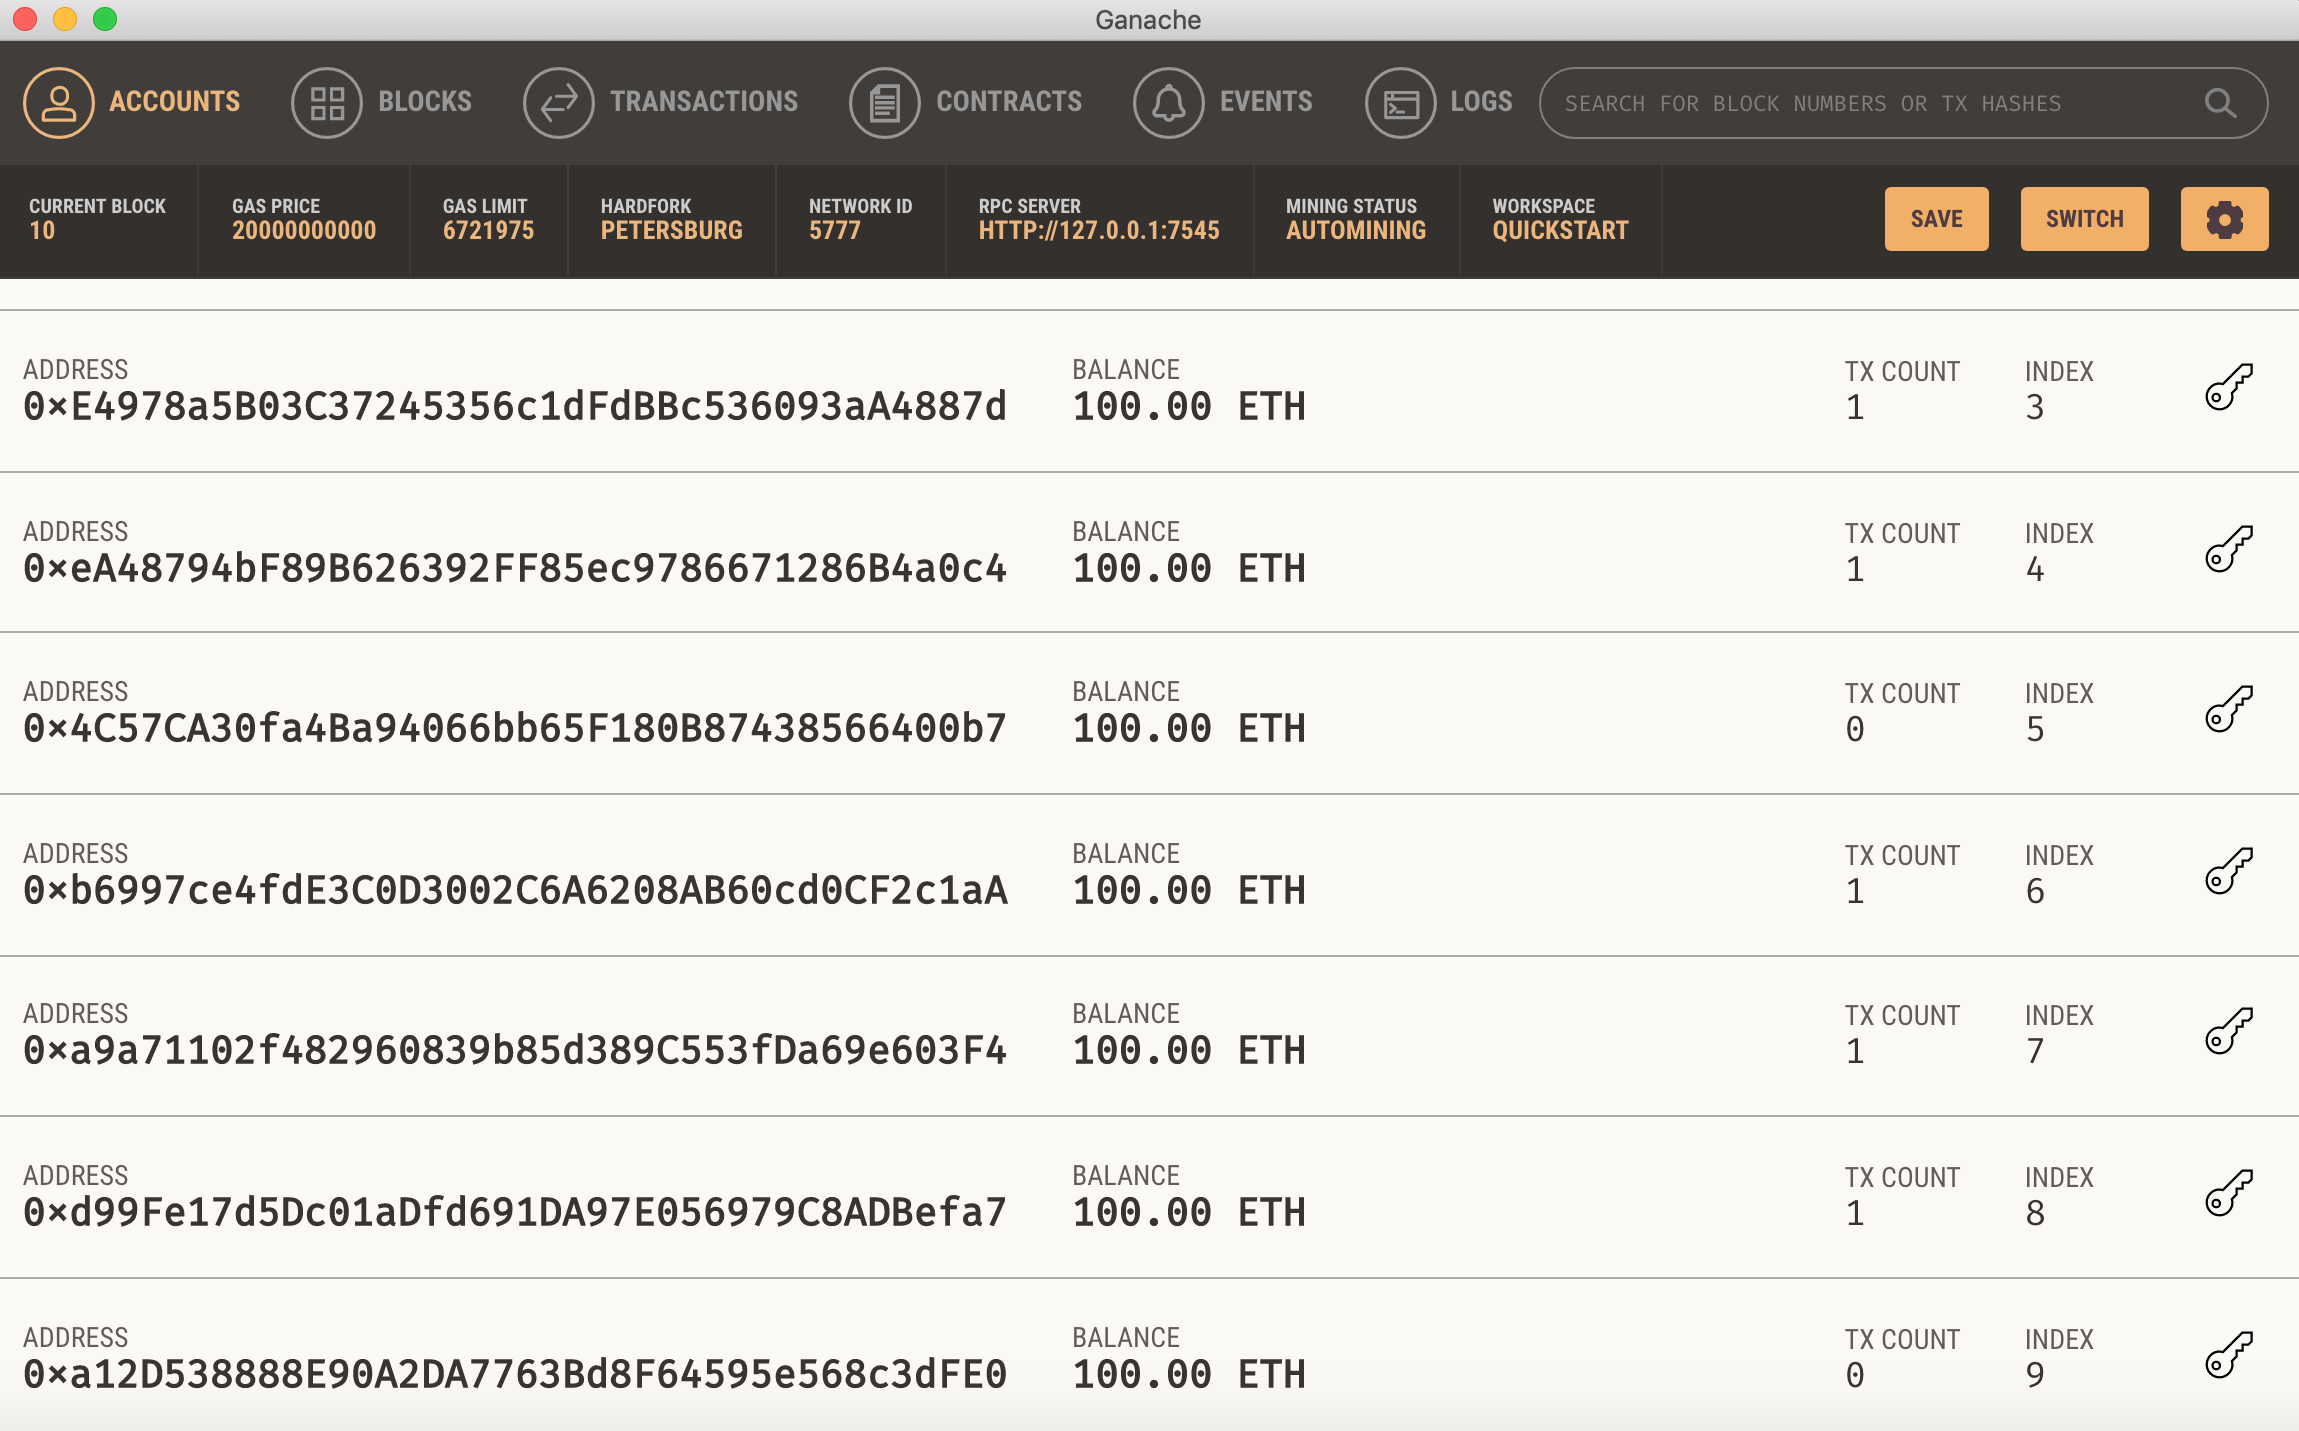
\includegraphics[width=\linewidth]{img/ganache-blockchain.png}
		\caption{Een Lokale blockchain opgezet via Ganache}
		\label{fig:ganache-blockchain}
	\end{figure}
	
	
	\subsection{Metamask}
	Metamask\footnote{Metamask is verkrijgbaar via https://metamask.io of via https://chrome.google.com/webstore} is een Ethereum wallet plugin voor Google Chrome die gebruikers toelaat om transacties van Ethereum dApps uit te voeren in de browser, zonder zelf een node moeten zijn in het netwerk. Door Metamask te installeren hoeft men met andere woorden de volledige blockchain dus niet meer te downloaden. 
	
	Voor deze implementatie is Metamask van cruciaal belang gezien het verantwoordelijk is voor de verificatie van Ethereum accounts. Daarnaast is het ook een zeer handige tool wanneer we onze implementatie in de browser willen testen, het laat ons toe om zeer snel tussen verschillende accounts te verspringen.
	
	Eenmaal de plugin geïnstalleerd is dient men een paswoord te creëren, daarnaast krijgt men ook een fallback sleutel
	
	\begin{figure}
		
\includegraphics[width=\linewidth]{img/metamask-truffle-ganache.png}
		\caption{Truffle, Metamask en Ganache logo's}
		\label{fig:metamask-truffle-ganache}
	\end{figure}
	\newpage
\section{Implementatie Smart Contracts}
	Eenmaal al de verschillende tools en plugins uit sectie \ref{sec:benodigdheden} geïnstalleerd zijn kan men aan het ontwikkelen van smart-contracts beginnen. In de volgende subsecties volgt de implementatie van een blockchain gebaseerd stemsysteem op basis van smart-contracts. Het volledige project kan gevonde worden op Github\footnote{Zie: https://github.com/Ocean97Li/bachelorproef/tree/master/poc/EthereumVote/backend} We beginnen met een simpele implementatie die niet self-tallying is. In een latere sectie zullen we de nodige cryptografie toevoegen om een systeem gelijkaardig aan het Open Network Protocol van  \textcite{McCorry2017} te bekomen.
	\subsection{Opzet Truffle}
	Voor we beginnen met het ontwikkelen van onze smart-contracts moeten we eerst een ontwikkelomgeving opzetten. Voor een vlotte start maken we gebruik van één van de template projecten beschikbaar via Truffle. 
	
	Na te navigeren naar een gewenste directory, gebruikt men het console commando: 
	 \lstset{language=bash}
	\begin{lstlisting}[numbers=none]
	> truffle unbox pet-shop
	\end{lstlisting}
	
	Dit creëert een nieuw project in de huidige directory, we openen het in een code-editor (Bijvoorbeeld VS-code). Figuur \ref{fig:truffle-template} toont de structuur van de genereerde Truffle template. Het project bevat momenteel zowel een back-end gedeelte (smart-contract) als een front-end (een javascript project). 
	
	In deze handleiding zullen we, met het principe van herbruikbaarheid in gedachten, de code opsplitsen in aparte front- en back-end projecten, de folder en inhoud onder \textit{\slash src}, als ook de afbeeldingen \textit{box-img-lg.png} en \textit{box-img-sm.png} mogen dus uit dit project verwijderd worden.
	
	Het project kan nu als start-template worden gebruikt voor onze implementatie.
	
	\begin{figure}
		\centering
		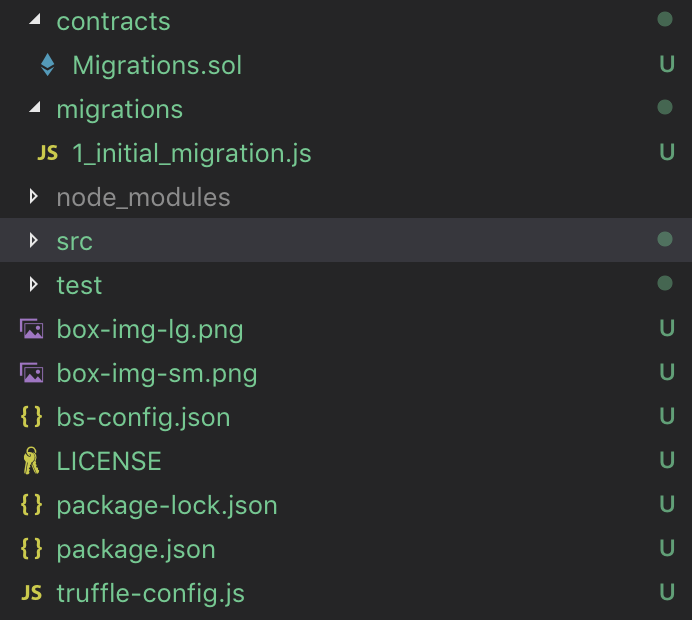
\includegraphics[width=\linewidth/2]{img/truffle-template.png}
		\caption{De structuur van een Ethereum Truffle project}
		\label{fig:truffle-template}
	\end{figure}
	
	\subsection{Basis implementatie}
	We beginnen met het aanmaken van een nieuw smart-contract bestand binnen het template-project. Dit doen we op de locatie \textit{contracts\slash Election.sol}. We overwegen de vereisten voor onze implementatie. Om een simpel stemsysteem te implementeren in een smart-contract hebben we nodig:
	\begin{itemize}
		\item een lijst van de `opties' waarop gestemd kan worden
		\item een lijst van de accounts die gestemd hebben
		\item per optie het aantal stemmen
	\end{itemize}
	Uiteraard zijn er verschillende manieren waarop we dit kunnen aanpakken. In de context van smart-contracts is het echter cruciaal dat we zo weinig mogelijk code schrijven. We baseren ons daarom op de implementatie die wordt gegeven door \textcite{McCubin2019}.\footnote{Zie ook https://github.com/dappuniversity/election}
	
	We beginnen met het declareren van de Solidity versie:

	\lstset{language=JavaScriptSolidity} 
	\begin{lstlisting}[numbers=none]
	pragma solidity ^0.5.8;
	\end{lstlisting}
	\lstset{language=JavaScriptSolidity} 

	Vervolgens starten we met het definiëren we van ons smart-contract \textit{Election} :
	\begin{lstlisting}[numbers=none]	
	contract Election {
		constructor () public {
		}
	}
	\end{lstlisting}
	
	Omdat we een lijst van de `opties' willen hebben en ook per optie willen bijhouden hoeveel stemmen er voor zijn, maken we gebruik van een custom type dat we \textit{Candidate} noemen. 

	Onze verkiezing hoeft niet per se om het verkiezen van een persoon te gaan, het is echter wel handig om over de opties te denken in termen van`kandidaten'. 
	Iedere optie is een kandidaat die een id, een `naam' (de optie tekst) en een aantal voorkeursstemmen heeft. 
	
	In Solidity definiëren we zo'n custom type in de vorm van een \textit{struct}:
	
	\begin{lstlisting}[numbers=none]	
	struct Candidate {
		uint id;
		string name;
		uint votes;
	}
	\end{lstlisting}
	
	We breiden \textit{Election} nu ook uit met de volgende attributen:
	
	\begin{lstlisting}[numbers=none]
	//Fetch the candidates	
	mapping(uint => Candidate) public candidates;
	// Store accounts that have voted
	mapping(address => bool) private voters;
	// Read candidate
	uint public candidatesCounter;
	\end{lstlisting}
	
	Het \textit{mapping} keyword in Solidity duidt een hashTable aan, in Solidity is dit de aangeraden verzameling-structuur\footnote{Zie https://ethereum.stackexchange.com/questions/2592/store-data-in-mapping-vs-array\#answer-2597}.  Mappings laten ons toe om key-value searching te doen. In het geval van  \textit{candiates} mappen we de `kandidaten' op basis van hun id's, die zijn numeriek en incrementeel. We houden het aantal kandidaten bij in \textit{candidatesCounter} zodat we niet onnodig in de mapping moeten zoeken, maar exact weten wat de range van id's is.
	
	Bij het attribuut \textit{voters} mappen we de adressen van alle kiezers op een booleaanse-waarde. Wensen we te weten of een kiezer reeds een stem uitgebracht, dan kunnen we dit via het \textit{voters} attribuut eenvoudig verifiëren. 
	
	We voegen een methode toe aan \textit{Election} die ons instaat stelt om  \textit{candiates} toe initialiseren:
	
	\begin{lstlisting}[numbers=none]
	function addCadidate(string memory _name) private {
		candidatesCounter++;
		candidates[candidatesCounter] = Candidate(candidatesCounter,_name,0);
	}
	\end{lstlisting}
	Merk op dat parameter in de bovenstaande functie gemarkeerd is met het Solidity \textit{memory} keyword. Dit duidt aan dat deze parameter niet in de blockchain dient opgeslagen te worden, de tegenhanger van dit keyword is \textit{storage}.
	
	Voorlopig zullen we onze opties `hardcoden' in de constructor functie, we kiezen voor een implementatie met simpele binaire ja/nee vragen:
	
	\begin{lstlisting}[numbers=none]
	constructor () public {
		addCadidate("Yes");
		addCadidate("No");
	}
	\end{lstlisting}
	
	Nu we opties hebben toegevoegd waarop gestemd kan worden rest ons enkel nog het implementeren van een stem functie. 
	
	Gebruikers mogen niet meermaals een stem uitbrengen, daarom controleren we iedere gebruiker die probeert te stemmen. 
	
	\begin{lstlisting}[numbers=none]
	function hasVoted() public view returns (bool ok) {
		return voters[msg.sender];
	}
	\end{lstlisting}
	
	Merk ook op dat hier wordt gebruik gemaakt van het Solidity \textit{view} keyword, dit duidt aan dat de betreffende functie geen aanpassingen zal maken aan het contract. 
	
	\begin{lstlisting}[numbers=none]
	function vote(uint _candidateId) public {
		if(!hasVoted()) {
			// Record voter has voted
			voters[msg.sender] = true;
			// Update candidate vote count
			candidates[_candidateId].votes++;
		}
	}
	\end{lstlisting}
	
	We vinden de kandidaat waarvoor de gebruiker stemde op basis van de parameter\textit{\_candidateId}. Door deze waarde in te vullen in de mapping \textit{candidates} krijgen we toegang tot de correcte Candidate struct. We verhogen het \textit{votes} attribuut van deze struct met 1. Op dit punt is de stem uitgebracht, we hebben nu een eenvoudig stemsysteem bekomen!
	
	De volledige code voor het smart contract is momenteel:
	
	\lstset{language=JavaScriptSolidity} 
	\begin{lstlisting}[frame=single,  label={lst:election}] 
	pragma solidity ^0.5.8;
	
	contract Election {
		// Store candidate
		struct Candidate {
			uint id;
			string name;
			uint votes;
		}
		
		//Fetch the candidates
		mapping(uint => Candidate) public candidates;
		
		// Store accounts that have voted
		mapping(address => bool) private voters;
		
		// Read candidate
		uint public candidatesCounter;
		
		// Constructor
		constructor () public {
			addCadidate("Yes");
			addCadidate("No");
		}
	
		function addCadidate(string memory _name) private {
			candidatesCounter++;
			candidates[candidatesCounter] = 
			Candidate(candidatesCounter,_name,0);
		}
		
		function hasVoted() public view returns (bool ok) {
			return voters[msg.sender];
		}
		
		function vote(uint _candidateId) public {
			if(!hasVoted()) {
				// Record voter has voted
				voters[msg.sender] = true;
				// Update candidate vote count
				candidates[_candidateId].votes++;
			}
		}
	}

	\end{lstlisting}
	
	
	\subsection{Migration toevoegen}
	Nu we een functioneel smartcontract hebben wensen we dit op onze lokale blockchain te deployen. Hiertoe dienen we  eerst een nieuw migration bestand aan het project toe te voegen op de locatie \textit{migrations\slash 2\_deploy\_contracts.js}.  
	
	Het een nieuwe bestand krijgt de volgende inhoud:
	
	\begin{lstlisting}[frame=single]
	// Find smart contract
	var Election = artifacts.require("./Election.sol");
	
	module.exports = function(deployer) {
	// List all the smart contracts to be deployed
		deployer.deploy(Election);
	};
	\end{lstlisting}
	
	De bovenstaande code zal ervoor zorgen dat Truffle  het `Election' smart contract op de blockchain kan plaatsen wanneer we het project deployen.
	
	\subsection{Truffle project linken aan Ganache}
	
	Om een beter overzicht te krijgen van de `state' van de lokale blockchain kunnen we ons Truffle project in Ganache toevoegen. Dit doen we door binnen Ganche naar de menu-optie `Contracts' te navigeren, vervolgens voor de optie `link truffle  projects'  te kiezen, naar het project te navigeren en daar het bestand \textit{truffle.js} aan te duiden. Tenslotte  kiezen we voor `save and restart'. Als we nu naar de menu-optie `Contracts' gaan krijgen we een overzicht van de contracten en hun status (\ref{fig:contracts-ganache1}).
	
	\begin{figure}
		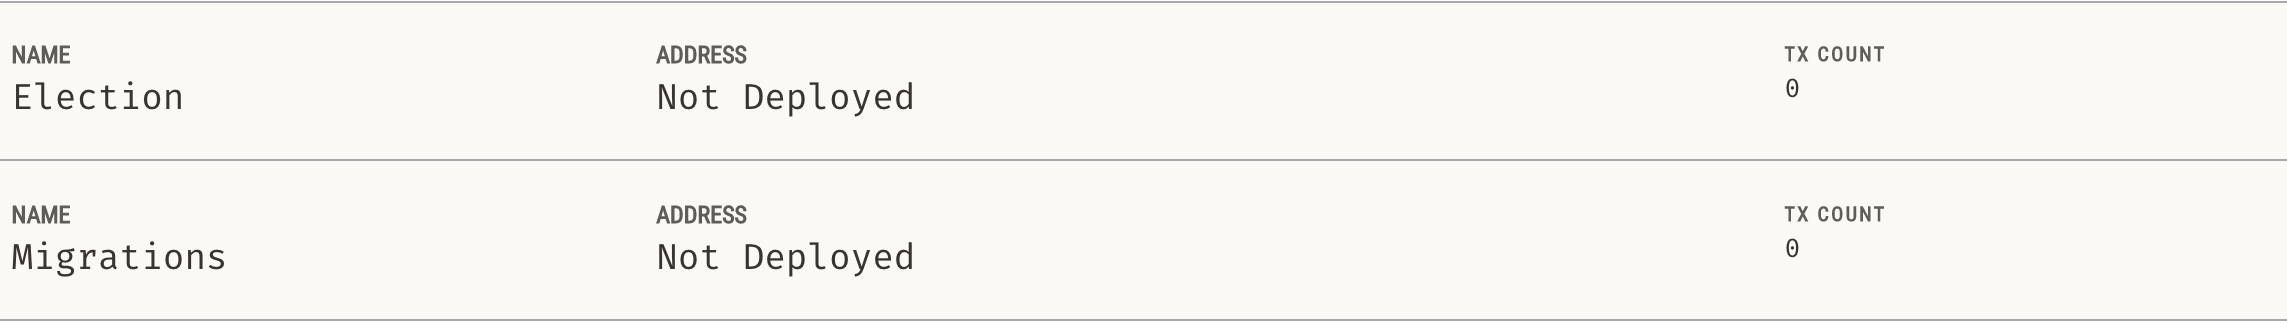
\includegraphics[width=\linewidth]{img/contracts-ganache1.png}
		\caption{De status van smart contracts weergegeven in Ganache}
		\label{fig:contracts-ganache1}
	\end{figure}
	
	
	\subsection{Deployen van smart contracts}
	
	Eenmaal we een migration file hebben voor onze smart-contracts, kunnen we deze deployen. Als de Ganache blockchain opgestart is en het truffle project eraan gelinkt, navigeren we naar het project in de console om vervolgens het volgende console commando te gebruiken:
	
	\begin{lstlisting}[numbers=none]
	> truffle migrate
	\end{lstlisting}
	
	Merk op dat indien we nu opnieuw wensen te deployen (in dit geval niet erg omdat we op een lokale blockchain werken) we het volgende commando dienen te gebruiken:
	
	\begin{lstlisting}[numbers=none]
	> truffle migrate --reset
	\end{lstlisting}
	
	Wanner er geen compilatie fouten aanwezig zijn in de code van de smart contracts kan er met succes deployed worden. In dat geval krijgt men voor ieder van de smart contracts een \textit{transaction receipt}:
	\lstset{language=bash}
	\begin{lstlisting}[numbers=none]
	 Deploying `Election'
	--------------------
	> transaction hash:    0xaf22d8d9c9c9a1230e1764d7a3bd9249a3...eb8fa
	> Blocks: 0            Seconds: 0
	> contract address:    0xBF1917F9c9cFee73A4E653de5ad62a6515b78Ed4
	> block number:        3
	> block timestamp:     1560958652
	> account:             0xE03c3692FED9D4f2cBc7c5a30b05Ae9ce7b3b839
	> balance:             99.98553468
	> gas used:            419914
	> gas price:           20 gwei
	> value sent:          0 ETH
	> total cost:          0.00839828 ETH
	
	
	> Saving migration to chain.
	> Saving artifacts
	-------------------------------------
	> Total cost:          0.00839828 ETH
	\end{lstlisting}
	
	Als we de contracts nu in Ganache bekijken zien we dat de status ook daar veranderd is naar deployed. (Zie Figuur \ref{fig:contracts-ganache2})
	
	\begin{figure}
		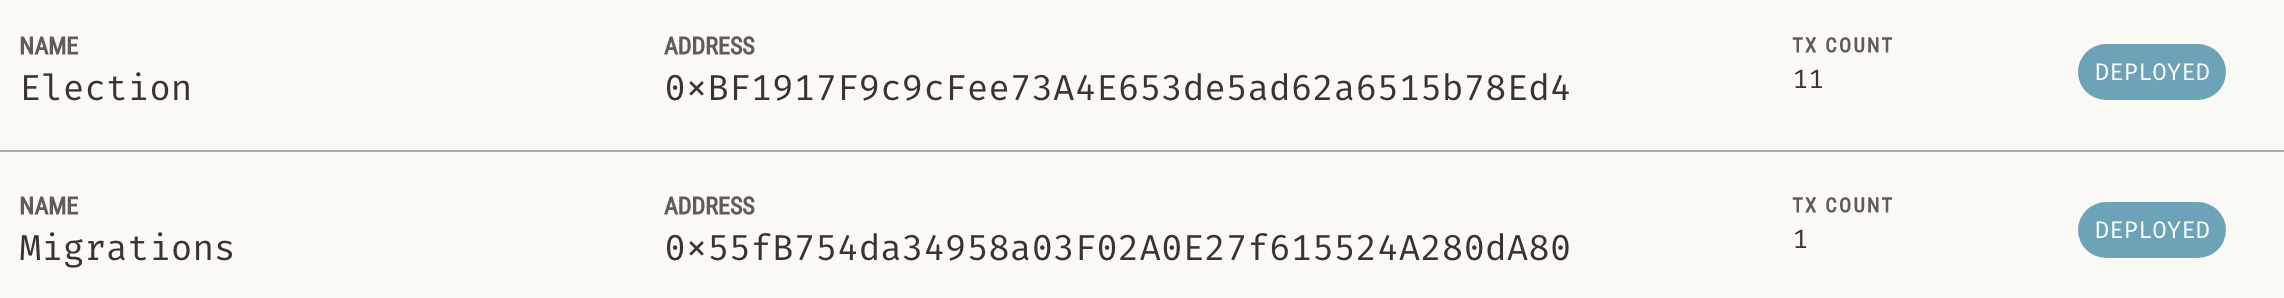
\includegraphics[width=\linewidth]{img/contracts-ganache2.png}
		\caption{Smart contracts deployed weergegeven in Ganache}
		\label{fig:contracts-ganache2}
	\end{figure}
	
	\subsection{Belang van testen}
	Bij het ontwikkelen van dApps speelt testen een cruciale rol. Eenmaal deployed naar een officieel netwerk kunnen functies die bugs bevatten en onverwacht gedrag vertonen erg kostelijk zijn voor gebruikers. Het is daarom best practice om enkel smart contracts te deployen die functioneel-volledig en getest zijn.  Doordat alles wat in de blockchain wordt bewaard immutable is, betekent het herdeployen van een smart-contract eigenlijk dat het huidige contract wordt vervangen door een nieuwe kopie. Zowel de state als het adres van het oude contract gaan verloren. Dit is brekend voor iedere front-end applicatie die aan de dApp verbonden is. 
	
	Door smart-contracts grondig te testen kunnen we dergelijke situaties vermijden.
	
	Er zijn verschillende methoden die men kan toepassen om een smart-contract te testen, standaard is om ze te schrijven in Solidity. Voor dit voorbeeld zullen we echter gebruik maken van Javascript. Via Truffle kunnen we met behulp van Javascript de  interacties van gebruikers met onze smart-contracts gemakkelijk simuleren. Truffle bevat immers standaard Mocha\footnote{Apart verkrijgbaar via https://mochajs.org} (testframework) en Chai Assertion Library\footnote{Apart verkrijgbaar via https://www.chaijs.com}. Deze twee tools stellen ons instaat om onze smartcontracts te importeren binnenin Javascript-testen. 
	
	
	\subsection{Smoke  test}
	We voegen een nieuw bestand toe op de locatie \textit{test\slash election.js}. We schrijven een smoke test, een test die nagaat of het smart-contract op correcte wijze geïnitialiseerd wordt.

	 \lstset{language=JavaScriptSolidity} 
	 \begin{lstlisting}
	 var Election = artifacts.require("./Election.sol");
	 	
	 contract("Election", function(accounts){
		var electionInstance;
		 
		it("Initializes two candidates", function() {
		 	return Election.deployed().then(function(instance){
		 		return instance.candidatesCounter();
		 	}).then(function(count){
		 		assert.equal(count,2);
		 	});
	 	});
	 	
		it("Initializes yes and no", function() {
	 		return Election.deployed().then(function(instance){
	 			electionInstance = instance;
	 			return electionInstance.candidates(1);
	 		}).then(function(candidate){
				assert.equal(
			 	candidate[0],1,"has the correct id: 1"
			 	);
				assert.equal(
				 	candidate[1],"Yes","has the correct value: `Yes'"
				);
				assert.equal(
				 	candidate[2],0,"has the correct amount of votes: 0"
				);
				return electionInstance.candidates(2);
	 		}).then(function(candidate){
				assert.equal(
					candidate[0],2,"has the correct id: 2"
				);
				assert.equal(
					candidate[1],"No","has the correct value: `No'"
				);
				assert.equal(
					candidate[2],0,"has the correct amount of votes: 0"
				);				
	 		}); // End function
	 	}); // End it()
	}); // End contract
	\end{lstlisting}
	
	Concreet testen we hier dat na instantiatie:
	\begin{itemize}
		\item Het attribuut \textit{canidatesCounter} = 2 is.
		\item Het attribuut \textit{candiates[0]} een `kandidaat' is met id = 1, naam = ``Yes'' en aantal stemmen = 0.
		\item Het attribuut \textit{candiates[1]}  een `kandidaat' is met id = 2, naam = ``No'' en aantal stemmen = 0.
	\end{itemize}
	\subsection{Testen uitvoeren}
	Om geschreven testen uit te voeren navigeren we naar de project-directory en gebruiken we het console commando:
	
	\begin{lstlisting}[numbers=none]
	> truffle test
	\end{lstlisting}
	
	Truffle voert hierop de al de testen binnen de directory \textit{test\slash} uit:
	
	\begin{lstlisting}[numbers=none]
	> Artifacts written to /var/folders/xq/mnnky8qn6c58pt33xhpz2bhw0000gn/T/test-119519-4744-y0zb1c.1il0l
	> Compiled successfully using:
	- solc: 0.5.8+commit.23d335f2.Emscripten.clang
	
	
	
	Contract: Election
	v Initializes two candidates
	v Initializes yes and no (93ms)
	
	
	2 passing (173ms)
	\end{lstlisting}
	
	De smoke test slaagt.
	
	\subsection{Testen in de Truffle console}
	Uiteraard dienen we  ook testen te schrijven voor de stem-functionaliteit. Gezien dit onderdeel van de code echter nog aan veranderingen onderworpen zal worden is het misschien voordeliger om de huidige werking op een andere manier te verifiëren. In plaats van een test te schrijven, kunnen we via de \textit{Truffle console} de toestand van de lokale blockchain bekijken.
	
	In de console navigeren we naar het project, vervolgens gebruiken we het console commando:
	
	\begin{lstlisting}[numbers=none]
	> truffle console
	\end{lstlisting}
	
	Dit opent de Truffle console. 
	Hier geven we het volgende commando in:

	\begin{lstlisting}[numbers=none]
	truffle(development)> Election.deployed()
		.then(function(i){app = i})
	\end{lstlisting}
	
	Indien het Election contract deployed is, wordt er een asynchrone callback-functie uitgevoerd.  De functie in kwestie krijgt  een instantie van Election (i) mee als parameter en maakt deze toegankelijk door ze in hem variabele op te slaan.
	Eenmaal de asynchrone code uitgevoerd is, hebben we via \textit{app} toegang tot de attributen en functies van het smart contract Election.
	
	Gezien we de stemfunctionaliteit willen testen, zullen we de stemfunctie \textit{vote()} oproepen.
	
	Hiervoor hebben we echter het publieke adres van één van de Ganache accounts nodig. Deze adressen kan men vinden in Ganache zelf, of bekomen via het Truffle console commando:
	\begin{lstlisting}[numbers=none,language=bash]
	truffle(development)>web3.eth.getAccounts()
	[ `0xE03c3692FED9D4f2cBc7c5a30b05Ae9ce7b3b839',
	`0xe60c19f8a1baC541483e303Dc3d9B4e28d580980',
	`0x47B7B70802E9eC6a5Df8570962574894f0Ac4c15',
	`0xE4978a5B03C37245356c1dFdBBc536093aA4887d',
	`0xeA48794bF89B626392FF85ec9786671286B4a0c4',
	`0x4C57CA30fa4Ba94066bb65F180B87438566400b7',
	`0xb6997ce4fdE3C0D3002C6A6208AB60cd0CF2c1aA',
	`0xa9a71102f482960839b85d389C553fDa69e603F4',
	`0xd99Fe17d5Dc01aDfd691DA97E056979C8ADBefa7',
	`0xa12D538888E90A2DA7763Bd8F64595e568c3dFE0' ]
	\end{lstlisting}
	
	We kopiëren een adres naar keuze en vullen dit in als \textit{from} property van de 2e parameter. Op deze manier versturen we een transactie vanuit de console, in naam van het geselecteerde adres. De 1e parameter is het id van de `kandidaat' waarvoor we stemmen.
	\begin{lstlisting}[numbers=none,language=bash]
	truffle(development)> app.vote(1,
		{ from: `0xE03c3692FED9D4f2cBc7c5a30b05Ae9ce7b3b839'}
	)
	\end{lstlisting}
	
	Ook hier krijgen we een \textit{transaction receipt.} Ook in Ganache zien we dat er een  nieuwe transactie heeft plaats gevonden (Figuur \ref{fig:contracts-ganache3})
	\begin{figure}
		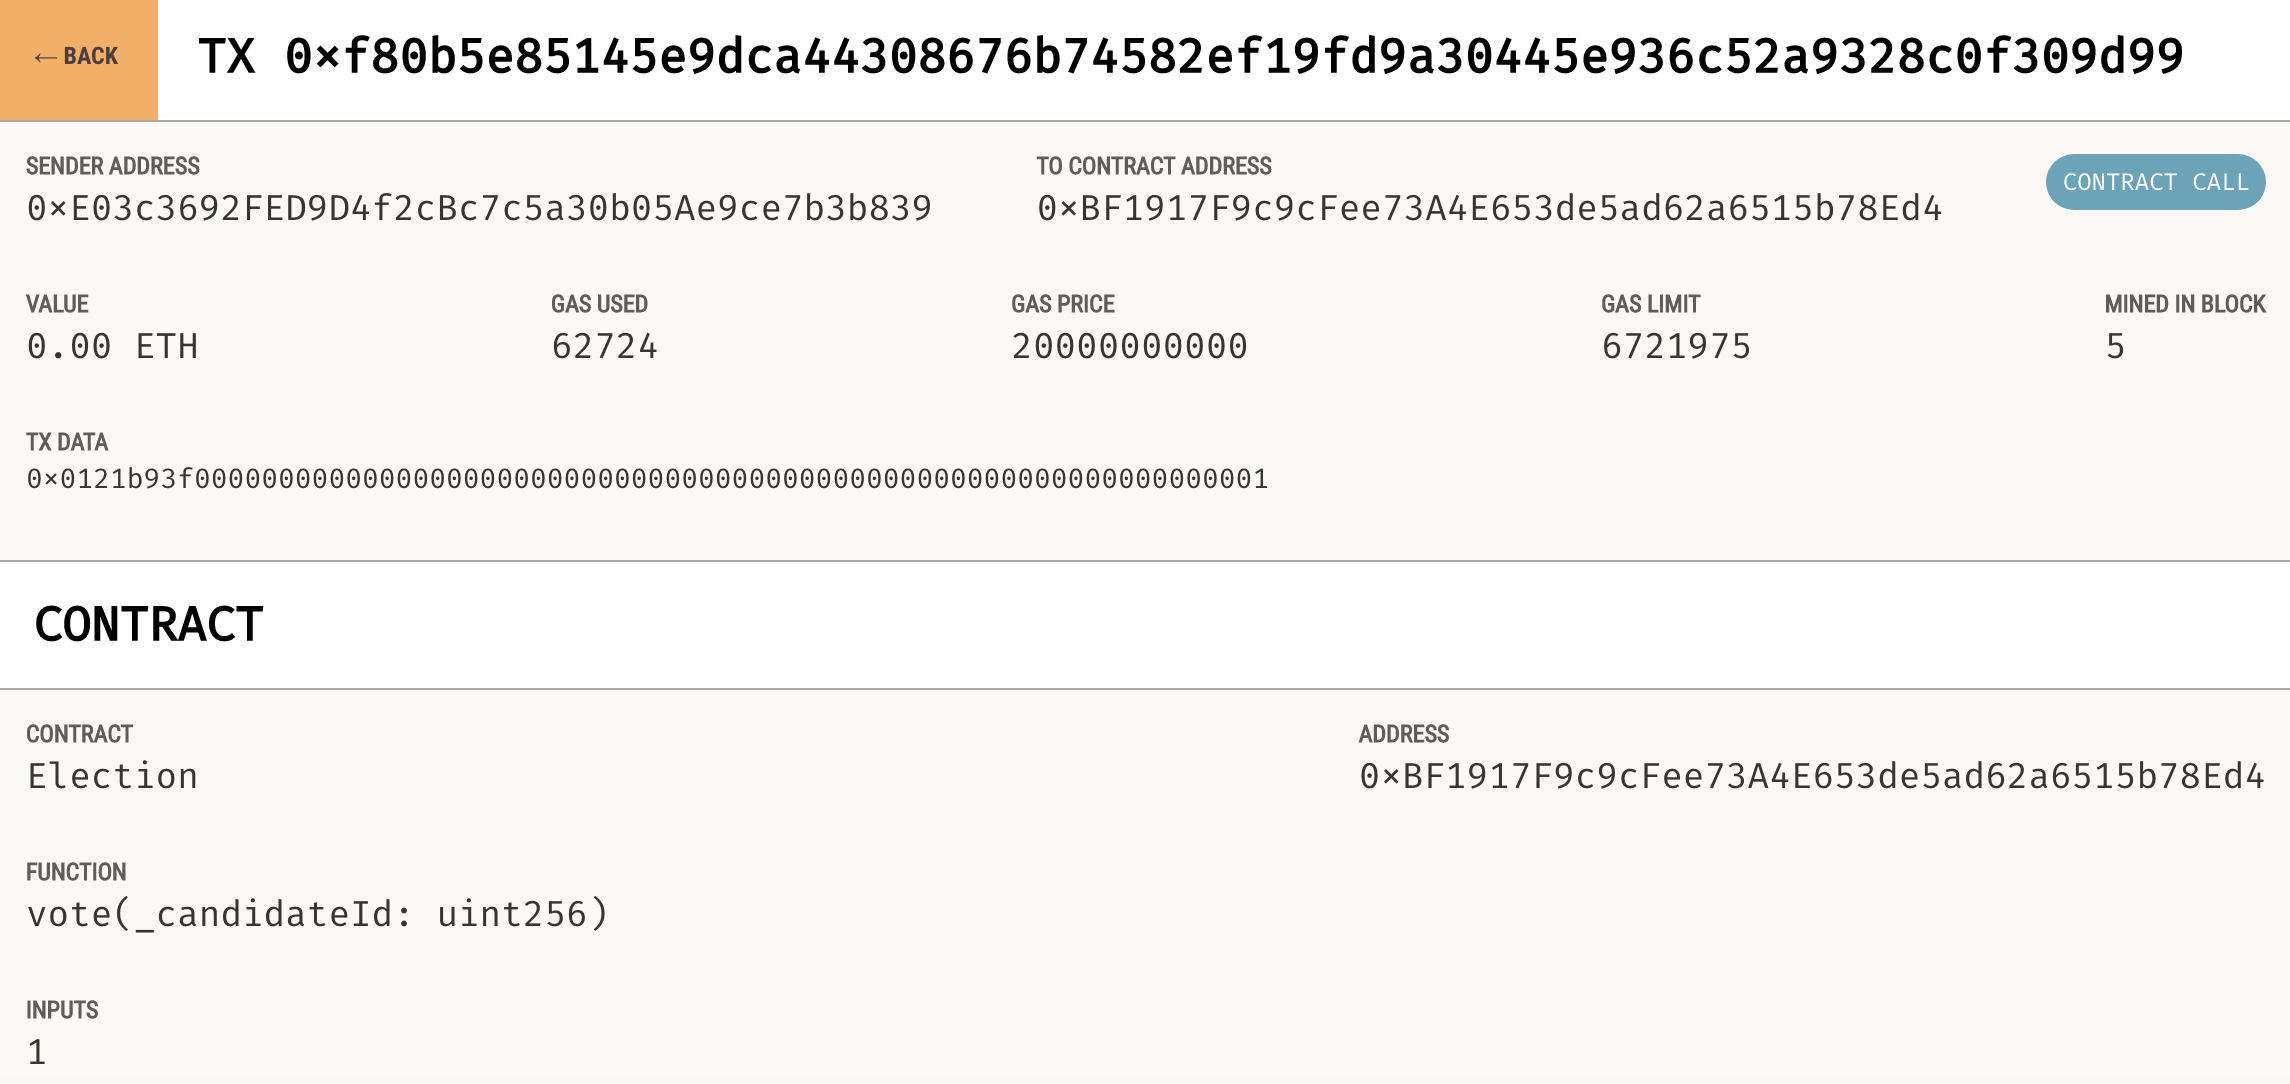
\includegraphics[width=\linewidth]{img/contracts-ganache3.png}
		\caption{Vote functie aangeroepen weergegeven in Ganache}
		\label{fig:contracts-ganache3}
	\end{figure}
	Om te controleren of er een stem is bijgekomen voor de gekozen optie geven we de volgende Truffle console commando's in:
	\begin{lstlisting}[numbers=none]
	truffle(development)> app.candidates(1)
	truffle(development)> app.candidates(2)
	\end{lstlisting}
	
	Dit resulteert in:
	\begin{lstlisting}[numbers=none,language=bash]
	Result {												Result {
	...															...
	id: <BN: 1>,										id: <BN: 2>,
	name: `Yes',									  name: `No',
	votes: <BN: 1> }							  votes: <BN: 0> }
	\end{lstlisting}
	
	Voor de eerste optie (`Yes') zien we dat er onder het attribuut \textit{votes} de waarde <BN: 1> staat. Het aantal stemmen hier is met andere woorden 1.
	Voor de tweede optie (`No') is dat niet het geval, \textit{votes} heeft de  waarde <BN: 0>. Het aantal stemmen hier dus onveranderd, 0.
	
	Dit toont aan dat onze stem-functie wel degelijk werkt!
	
	Merk wel op dat in de huidige implementatie totaal geen garantie biedt op het vlak van anonimiteit. Het enigste wat de anonimiteit van een kiezer enigszins beschermt is de abstracte aard van accounts, de kiezer is alleen bekend via zijn Ethereum adres. 
	
	\subsection{Ethereum en geheimen bewaren}
	Een van de moeilijkheden waarmee men te maken krijgt tijdens ontwikkelen van gedecentraliseerde applicaties binnen Ethereum, is het feit dat het zeer moeilijk is om anonimiteit of privacy voor gebruikers te creëren. De aard zelf van de blockchain-technologie legt immers de nadruk op het publiek beschikbaar maken van alle gegevens. In Ethereum zien we dit zeer sterk, iedere transactie en al de daar bijhorende parameters zijn publiek.  Bovendien gaat het veel verder dan alleen transacties. Eigenlijk is alles publiek binnen de Ethereum-blockchain. Private attributen en methoden mogen dan wel bestaan, de waarden zullen nog steeds publiek zichtbaar zijn. \autocite{Buterin2014}
	
	Voor onze implementatie vormt dit een potentieel probleem, gezien we een stem als parameter wensen door te geven. Op het vlak van stemsystemen is anonimiteit van kiezers  vaak noodzakelijk. Gezien Ethereum geen private transacties ondersteund (sommige blockchains doen dit wel)  moeten we op zoek gaan naar alternatieve methodes. Het lijkt een logische om te kijken of we de stem van de kiezer die we doorgeven als parameter niet kunnen encrypteren. Het probleem is echter dat standaard encryptie en decryptie technieken niet zullen werken op de blockchain. We kunnen immers geen enkel geheim bewaren op de blockchain,  decryptie sleutels zijn dus ook onmogelijk.
	
	Het gevolg is dus dat we geen keuze hebben dan gebruik moeten maken van  geavanceerde cryptografische technieken, willen we ons systeem volledig veilig maken. Een mogelijke cryptografische techniek de we hier zouden kunnen toepassen is die van het OVNP van \textcite{McCorry2017} dat we in het vorige hoofdstuk bespraken. Dit blijkt echter in de praktijk zeer moeilijk te doen. In een volgende sectie zullen we hier verder op ingaan.	
	
	\begin{figure}
		\centering
		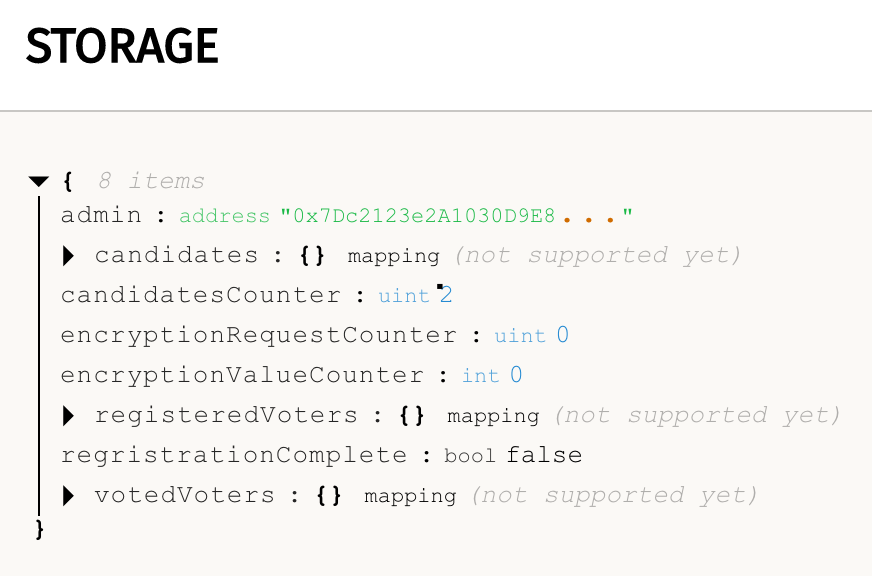
\includegraphics[width=\linewidth/2]{img/contracts-ganache4.png}
		\caption{Alle attributen van een contract zijn publiek zichtbaar}
		\label{fig:contracts-ganache4}
	\end{figure}

	\section{Front-end applicatie}
	Eenmaal we de basis we een werkende basis back-end hebben dienen we er natuurlijk ook nog een front-end applicatie voor te ontwikkelen. In deze handleiding zullen we gebruik maken van een Angular, een open source javascript-framework dat de ontwikkelaars instaat stelt om performante Single Page Applications te schrijven. We maken gebruik van Angular omdat de structurering  van de code bijzonder regide is, waardoor de functionaliteiten mooi opgesplitst zijn en de ontwikkelervaring bijzonder aangenaam.  Het staat de lezer echter vrij om een javascript-framework naar keuze te gebruiken, indien hij of zij dat wenst. Het gaat hier  niet zo zeer om de ontwikkeling van de front-end applicatie als om het maken van de verbinding tussen webapplicatie en Ethereum blockchain zodat we kunnen interageren met ons smart-contract. 
	
	\subsection{Opzet}
	Zoals gezegd zullen we een Angular project opzetten, lezers die gebruik wensen te maken van een ander Javascript-framework kunnen de komende stappen overslaan, zij hoeven enkel de vernoemde \textit{node\_modules } te installeren. 
	
	We beginnen met het installeren van de angular cli, deze zal ons toe laten om een angular project te maken.
	
	maken gebruik van het console commando:
	\begin{lstlisting}[numbers=none,language=bash]
	>npm install -g @angular/cli
	\end{lstlisting}
	Dit installeert de angular cli op een globaal niveau, vanaf nu kunnen we er overal gebruik van maken.
	
	We navigeren naar de directory waar we het front-end project willen aanmaken, vervolgens gebruiken we het console commando:
	\begin{lstlisting}[numbers=none,language=bash]
	>ng new EthereumVote
	\end{lstlisting}
	De angular cli zal nu een nieuw project voor ons creëren in de huidige directory. 
	
	Nu installeren we de nodige node\_packages:
	\begin{itemize}
		\item \textbf{web3.js}: een verzameling javascript libraries  die toelaten om te communiceren met Ethereum-instantie, hetzij via  een HTTP-, WebSocket- of IPC-verbinding.
	\end{itemize}
	
	
	
	
	
	
	Navigeer naar de hoofddirectory van het nieuwe project en maak een nieuwe directory `services':
	\begin{lstlisting}[numbers=none,language=bash]
	>mkdir services
	\end{lstlisting}
	Navigeer vervolgens naar die directory en 
	
	
	
	
	
	
	
	
	
	
	
	
	
	
	
	
	

	










% Voeg hier je eigen hoofdstukken toe die de ``corpus'' van je bachelorproef
% vormen. De structuur en titels hangen af van je eigen onderzoek. Je kan bv.
% elke fase in je onderzoek in een apart hoofdstuk bespreken.

%\input{...}
%\input{...}
%...

%%=============================================================================
%% Conclusie
%%=============================================================================

\chapter{Conclusie}
\label{ch:conclusie}
In deze scriptie werd een onderzoek gevoerd naar de haalbaarheid van blockchain gebaseerd stemmen, daarnaast werd ook de benodigde informatie voor het ontwikkelen van een dergelijk systeem  verzameld. De bijdrage en \textit{proof of concept} van deze scriptie werden gegeven in de vorm van een praktische handleiding waarin een \textit{decentralized application} - ofwel DApp -  genaamd EthereumVote werd ontwikkeld. 

 Dit onderzoek is bedoeld voor iedereen die geïnteresseerd is in zaken als burgerparticipatie, verkiezingen en democratie. Hoewel vaak technisch van aard is het geschreven met niet technisch-onderbouwde personen in gedachten. Alleen de handleiding verondersteld een technische achtergrond. Ze is specifiek gericht op ontwikkelaars met interesse in blockchain stemsystemen. De meerwaarde is dat een compleet stappenplan gegeven wordt, met extra uitleg over gebruikte tools, complexe code, enzovoort. Waar andere handleidingen een louter functionele focus hebben, is er bij EthereumVote rekening gehouden met anonimiteit en schaalbaarheid. Encryptie en registratie werden daartoe als `extra' stappen gebruikt, resulterend in een gulden middenweg tussen absolute veiligheid en kost-efficiëntie.
 
In dit finale het hoofdstuk wordt er een antwoord geformuleerd op de onderzoeksvragen waarrond deze scriptie gebouwd werd:
\begin{itemize}
	\item Wat zijn de voor- en nadelen van de blockchain-technologie in het kader van een stemsysteem?
	\item Is er sprake van een onoverkomelijk schaalbaarheidsprobleem voor blockchain-technologie?
	\item Welke tools heeft men nodig om een blockchain-gebaseerd stemsysteem op te zetten en wat zijn de voor- en nadelen hiervan?
	\item Is een blockchain-gebaseerd stemsysteem haalbaar in de praktijk?
\end{itemize}
\section{Verwachte resultaten en conclusies versus realiteit}
Bij aanvang van dit onderzoek werden resultaten verwacht gelijkaardig aan het onderzoek van \textcite{McCorry2017}. De verwachting was immers dat het werk van dit onderzoek beschikbaar zou zijn als code-bibliotheek. Tijdens de implementatie van EthereumVote bleek dit echter niet het geval, er kon dus ook niet op verder gebouwd worden. 

Veranderingen in de onderliggende technologie leidden dit onderzoek bovendien tot de conclusie dat een meer performante oplossing nodig was. De zeer simpele implementatie van \textcite{McCubin2019} werd daartoe gecombineerd met concepten uit het werk van \textcite{McCorry2017}. EthereumVote is dus niet het verwachte resultaat, het is een overwogen compromis: meer performantie in de ruil voor verlaagde veiligheid op vlak van anonimiteit. 

De algemene conclusies van dit onderzoek komen grotendeels overeen met de initiële verwachtingen.  Blockchain gebaseerde stemsystemen lijken inderdaad over een groot potentieel te beschikken maar worden - ook zoals verwacht - voornamelijk gehinderd  door een schaalbaarheidsprobleem. Dit onderzoek bevestigd hiermee ook de conclusies van zijn voorgangers. Het zijn conclusies die voorzichtig positief kunnen genoemd worden. Het beantwoorden van de onderzoeksvragen leverde deze scriptie bovendien ook enkele nieuwe inzichten op, deze zijn te lezen in de volgende secties.
\section{Voordelen en nadelen}
De vele voordelen van blockchain gebaseerde stemsystemen kwamen aan bod in sectie \ref{sec:blockchain-gebaseerd-stemmen}. Samengevat zijn blockchain gebaseerde stemsystemen  - indien correct geïmplementeerd - beter op het vlak van \textit{privacy}, \textit{transparantie},  \textit{fouttolerantie},  \textit{veiligheid} en \textit{correctheid} dan hedendaagse elektronische tegenhangers. Decentralisatie speelt daarbij een significante rol. Blockchain gebaseerde systemen hebben dus het potentieel om beter te zijn, maar zijn dit niet automatisch.
	
Verder aansluitend op het vorige punt, is het feit dat veel zogenaamde nadelen aan blockchain gebaseerd stemmen heel implementatie gebonden zijn. Sommige implementaties benutten bijvoorbeeld al het volle potentieel van blockchain als technologie, andere doen dit dan weer niet. 

In sectie \ref{sec:blockchain-gebaseerd-stemmen} lag de focus vooral op algemene, recurrente problemen. Een van de hoofdreden die  wordt gegeven is dat er te weinig ondersteuning is op bestaande blockchain platformen voor de ontwikkeling van stemsystemen. Er is voornamelijk een gebrek aan cryptografische ondersteuning, dat was ook de bevinding tijdens de \textit{proof of concept} van deze scriptie.
	
Om die reden lijkt het logisch dat men (voor grootschalige verkiezingsscenario's) een eigen blockchain netwerk opzet. Het grote nadeel hier is echter dat dit bijzonder kostelijk is, zowel op vlak van nodige infrastructuur als het verzamelen van technische kennis.
	
Tenslotte is er ook nog een veelbesproken probleem met blockchain en schaalbaarheid.
\section{Onoverkomelijk schaalbaarheidsprobleem}
 lijkt er sprake te zijn van een schaalbaarheidsprobleem voor blockchain technologie . Het is een probleem dat de ingebruikname van blockchain technologie in verschillende velden verhindert, ook in de context van stemsystemen is dit het geval. Het probleem komt voort uit de structuur van blockchains. 
 
 Zoals besproken in sectie \ref{sec:blockchain-gebaseerd-stemmen} zijn blockchains intrinsiek niet schaalbaar: De snelheid waaraan het toevoegen van blokken aan een keten via het \textit{proof of work} algoritme gebeurt zal altijd het aantal transacties dat per seconden kan worden verwerkt limiteren. 
 
 De complexiteit van \textit{proof of work} verlagen is vaak niet wenselijk gezien dit vaak tot minder decentralisatie leidt en dus de blockchain minder veilig maakt. Zonder twijfel is er sprake dus van een serieus schaalbaarheidsprobleem.
	
De vraag is nu of het schaalbaarheidsprobleem onoverkomelijk is, naar de toekomst toe. 
	
Het is onmogelijk om thans met zekerheid een antwoord op die vraag te bieden. Het is duidelijk dat er pogingen ondernomen worden om het probleem te trotseren: in sectie \ref{sec:ethereum-en-smart-contracts} bespraken we bijvoorbeeld Ethereum's oplossing in de vorm van een nieuw mining algoritme genaamd \textit{proof of stake}. Bitcoin lijkt het over een andere boeg te gooien met een oplossing in de vorm van \textit{off-chain} transacties. De toekomst zal moeten uitwijzen of deze inspanningen het probleem effectief zullen oplossen.
\section{Tools en ontwikkeling}
	
In deze scriptie werd EthereumVote voorgesteld als een zelf-geimplementeerd blockchain gebaseerd stemsysteem. De verschillende tools nodig voor de ontwikkeling van deze DApp kwamen aanbod in sectie \ref{sec:benodigdheden}, de mogelijke problemen die men ermee kan ondervinden werden besproken in hoofdstuk \ref{ch:methodologie}.
	 
Voor Truffle en Ganache is er nauwelijks van nadelen te spreken, beide tools werken uitstekend samen en stellen ontwikkelaars instaat om de werking van hun DApps op een lokale blockchain te simuleren. 

Ook bij de front-end tools Metamask en truffle-contracts zijn er niets dan voordelen. Metamask is een Ethereum wallet die ons instaat stelt om met het netwerk te interageren zonder zelf een node te zijn. Truffle contracts stellt ons instaat om een interface van het smart-contract aan te spreken in de front-end. 

De enige noemenswaardige problemen zijn te vinden bij web3, in de vorm van slecht onderhouden dependencies. In hoofdstuk \ref{ch:methodologie} van deze scriptie werden de daaruit volgende comptabiliteitsproblemen beschreven. Hoewel dit zeker een minpunt is,  blijft web3 een essentiële tool voor de ontwikkeling van DAppps: met enkele lijnen code verbindt het de front-end applicatie met het Ethereum netwerk.
\section{Haalbaarheid}
Kleinschalige blockchain stemsystemen zijn technisch volledig haalbaar, de vele praktijk voorbeelden die werden aangehaald in sectie \ref{sec:blockchain-gebaseerd-stemmen} bevestigen dit. EthereumVote, voorgesteld in hoofdstuk \ref{ch:handleiding} van deze scriptie toont bovendien aan dat de ontwikkeling van een veilig en efficiënt stemsysteem niet complex of kostelijk hoeft te zijn.
	
De inherente schaalbaarheidsproblemen en het gebrek aan absolute veiligheid (op het vlak van anonimiteit) maken blockchain momenteel niet geschikt als onderliggende technologie voor grootschalige verkiezingen zoals we die kennen in de electorale politiek. Zelfs al zouden alle schaalbaarheidsproblemen van de technologie verholpen worden, dan nog zou de adaptatie in politieke verkiezingen erg moeilijk zijn.  Momenteel is er al veel kritiek op elektronisch stemmen, voor nieuwe technologieën zoals blockchain lijkt er alleen nog meer wantrouwen te heersen. 
	
Zolang er duidelijke nadelen verbonden blijven aan blockchain, kan de technologie niet doorbreken in de context van verkiezingen.  Zelfs als men zou kunnen concluderen dat een bepaald blockchain gebaseerd stemsysteem in zijn geheel voordeliger is dan de huidige elektronische en papieren stem (dewelke minder `perfect' zijn dan ze vaak worden uitgemaakt), dan nog blijft de ingebruikname zo goed als onmogelijk.
	
Het lijkt erop dat een praktisch onfeilbaar stemsysteem gepresenteerd moet worden alvorens blockchain zelfs maar in aanmerking kan komen als oplossing vanuit het politieke en juridische standpunt. Zo'n onfeilbaar systeem is volgens dit onderzoek met de huidige blockchain technologie moeilijk, als niet onmogelijk.  Er zou infeite een nieuwe, speciale variant van blockchain technologie moeten ontwikkelt worden. Projecten zoals het Moscow's Citizen's Initiative tonen immers aan dat er met voldoende politieke wil is en de juiste economische middelen al veel meer mogelijk is. 
	
De conclusie is dus dat grootschalige blockchain gebaseerde stemsystemen voorlopig niet haalbaar zijn en dat ook niet plots zullen worden. Potentieel naar de toekomst toe is er wel, alleen is het de vraag of de omstandigheden  (politiek, economisch, technologisch) het benutten er van zullen toelaten. Mocht dit het geval zijn dan ziet deze scriptie de toekomst van blockchain gebaseerde stemsystemen als een positieve zaak.
	
Verder onderzoek zou kunnen uitwijzen hoe groot het potentieel precies is. Concreet zou er een studie kunnen gevoerd worden naar het financiële aspect, waarin de totale kostprijs voor de opzet van een stemsysteem als ook het energie verbruik in operatie wordt berekent. Een andere studie die gevoerd zou kunnen worden is een vergelijkend onderzoek naar de verschillende manieren om anonimiteit   voor gebruikers te creëren. Het zou bijvoorbeeld bijzonder interessant zijn om verkiezingen op basis van hoogstaande cryptografische protocollen zoals OVNP en BroncoVote simultaan naast elkaar te draaien en de resultaten te vergelijken.
	
%% onderzoeksvra(a)g(en). Wat was jouw bijdrage aan het onderzoeksdomein en
%% hoe biedt dit meerwaarde aan het vakgebied/doelgroep? Reflecteer kritisch
%% over het resultaat. Had je deze uitkomst verwacht? Zijn er zaken die nog
%% niet duidelijk zijn? Heeft het onderzoek geleid tot nieuwe vragen die
%% uitnodigen tot verder onderzoek?




%%=============================================================================
%% Bijlagen
%%=============================================================================

\appendix

%%---------- Onderzoeksvoorstel -----------------------------------------------

\chapter{Onderzoeksvoorstel}

Het onderwerp van deze bachelorproef is gebaseerd op een onderzoeksvoorstel dat vooraf werd beoordeeld door de promotor. Dat voorstel is opgenomen in deze bijlage.

% Verwijzing naar het bestand met de inhoud van het onderzoeksvoorstel
%---------- Inleiding ---------------------------------------------------------

\section{Introductie} % The \section*{} command stops section numbering
\label{sec:introductie}Het democratisch stemmen is een cruciaal beslissingsmechanisme aanwezig in iedere laag van onze moderne samenleving, het vormt niet alleen de basis van het politieke systeem in vele landen, ook de bedrijfswereld is er van doordrongen. Stemprocessen zijn niet meer weg te denken uit de organisaties van vandaag. Of het nu gaat over besluiten op laag, functioneel niveau of over strategische beslissingen op hoog bestuurlijk niveau, de verantwoordelijkheid voor het maken van keuzes ligt steeds vaker bij een groep van mensen via een stemproces, dan bij één enkel individu. Het belang van stemmen op zowel economisch als politiek vlak valt dan ook  niet te onderschatten. De vraag die we onszelf echter moeten stellen is de volgende: hoe houdt men een proces waar zoveel van afhangt betrouwbaar, veilig en eerlijk? 
\linebreak{}
In de meeste gevallen blijkt het antwoord op die vraag vrij eenvoudig: waar het aantal participanten klein is, kan er gemakkelijk door iedere deelnemer of observator geverifieerd worden wat het resultaat van de stemming is. Iedere individuele deelnemer kan getuigen dat alles correct verloopt en dat maakt de kans op frauduleuze praktijken veel kleiner. Wordt het aantal participanten echter groter, dan is een dergelijk systeem onmogelijk. In zo'n geval bepaalt men het resultaat van de stemming door middel van een zogenaamde centrale autoriteit. Deze derde partij voert een controlerende functie uit en garandeert de betrouwbaarheid voor alle participanten. Bij nationale verkiezingen is dit bijvoorbeeld het stembureau. 
\linebreak{}
Het is van fundamenteel belang dat de centrale autoriteit neutraal is. Eén van de gevaren bij  dergelijke instanties is namelijk het risico op machtsmisbruik. Zo zijn voorafbepaalde of frauduleuze verkiezingen -hoewel bij ons gelukkig zeldzaam- niet ongekend. Een ander potentieel gevaar bij grote stemprocessen zijn onmoedwillige fouten. Er kunnen tal van menselijke of technische fouten optreden waardoor het resultaat van de stemming niet of niet geheel correct is. Een persoon die stemmen moet tellen kan fouten maken of een machine die stemmen moet registreren kan het laten afweten. Er is met andere woorden een probleem op het vlak van betrouwbaarheid. 
\linebreak{}
Een oplossing die een betrouwbaarder stemresultaat  garandeert lijkt de liggen in het digitaliseren van het proces. Bij digitalisatie krijgt men echter te maken met nieuwe risico's op het vlak van veiligheid, denk aan digitale fenomenen zoals: hacking, cyberaanvallen en identiteitsdiefstal. Toch zijn de voordelen die zijn verbonden aan digitalisatie immens: niet alleen op vlak van betrouwbaarheid, maar ook op vlak van efficiëntie, effectiviteit en gebruiksvriendelijkheid. Digitalisatie combineert zich echter zeer moeilijk met een centrale autoriteit: om het stemproces te digitaliseren zou men eigenlijk van het systeem van een centrale autoriteit moeten afstappen. 
\linebreak{}
Een mogelijkheid biedt zich aan in de vorm van de Blockchain technologie. Deze werd in feite net voor dit soort van problemen ontwikkeld. De oorsprong van deze technologie is namelijk gelinkt aan het ontstaan van 's werelds eerste gedecentraliseerde digitale munteenheid: de bitcoin. 
Net zoals dat bij het stemproces het geval is, wordt de legitimiteit van een reguliere munteenheid bepaald door een centrale autoriteit, in dit geval is dat de bank. Iedere (elektronische) transactie van geld gebeurt via deze autoriteit. De bitcoin is echter niet gelinkt aan een centrale bank, haar legitimiteit komt van een systeem dat blockchain wordt genoemd. De werking daarvan is in essentie niets meer dan de terugkeer naar een gedecentraliseerd systeem waarin iedere participant aan verificatie doet. 
\linebreak{}
Dit concept vormt de basis voor een systeem met een zeer hoog niveau van veiligheid en betrouwbaarheid. Omdat net dit de zaken zijn die bij stemprocessen van belang zijn, is een stemapplicatie op basis van blockchain zeker het onderzoeken waard.  De intentie van deze scriptie is dan ook antwoord te kunnen bieden op de volgende onderzoeksvragen:
\linebreak{}
\begin{itemize}
  \item Wat zijn de voor- en nadelen van de blockchain-technologie in het kader van een stemsysteem?
  \item Is er sprake van een onoverkomelijk schaalbaarheidsprobleem voor blockchain-technologie?
  \item Welke tools heeft men nodig om een blockchain-gebaseerd stemsysteem op te zetten en wat zijn de voor- en nadelen hiervan?
  \item Is een blockchain-gebaseerd stemsysteem haalbaar in de praktijk ?
\end{itemize}

%---------- Stand van zaken ---------------------------------------------------

\section{State-of-the-art}
\label{sec:state-of-the-art}

\subsection*{Blockchain 1.0: Bitcoin}
In dit eerste deel van de state-of-the-art wordt er een beeld geschetst van wat blockchain is en hoe het werkt achter de schermen. Dit wordt aan de hand van blockchain 1.0 gedaan, ofwel de originele blockchain-bitcoin-implementatie.
\subsubsection*{Wat is blockchain?}
 Blockchain is een gedecentraliseerde manier om gegevens op te slaan die voor het eerst geconceptualiseerd werd in de jaren negentig  ~\autocite{Dai1998} maar pas echt groot werd na de publicatie van ~\textcite{Nakamoto2008}. Het bijzondere aan de bitcoin-blockchain-implementatie is dat het peer-to-peer technologie combineert met wiskundige cryptografie, om tot een systeem te komen dat kan functioneren zonder de hulp van een vertrouwde derde partij  (centrale autoriteit) om de legitimiteit van iedere bitcoin te verifiëren. Blockchain werkt namelijk niet op basis van vertrouwen maar op basis van wiskundig bewijs.
 
 \subsubsection*{Hoe werkt het?}
Een blockchain is in datastructuur die bestaat uit een ketting van informatieblokken. Het is een ketting die fungeert als een soort publiek gedistribueerde boekhouding. Eenmaal informatie is opgeslagen in een blockchain, is het vrijwel onmogelijk om deze ongedetecteerd te wijzigen. Ieder blok van de ketting bestaat namelijk uit 3 velden: de data, de hash van het blok en de hash van het vorige blok. In het dataveld kan informatie worden opgeslagen. Het soort informatie dat men hier vindt is afhankelijk van de specifieke implementatie. In een bitcoin-blockchain wordt bijvoorbeeld een bitcoin-transacties opgeslagen. Ieder blok heeft daarnaast ook een hash, dit is een unieke identifier die wordt gegenereerd op basis van de inhoud van het blok. Iedere verandering aan het dataveld brengt ook een wijziging van de hashcode teweeg. Tenslotte is er nog het derde veld dat de hashcode van het vorige blok bijhoudt. Als iemand de data in één blok zou wijzigen, dan zou dit zorgen voor een aanpassing van de hash van dat blok. Het volgende blok bevat dan echter nog steeds een verwijzing naar de oorspronkelijke hash, die plots niet meer bestaat. De hashcode van het volgende blok kan dus niet  correct berekend worden. Ook de hashcodes van al de daarop volgende blokken kunnen bijgevolg niet meer correct berekend worden. Het gevolg is dus dat na een gecorrumpeerd blok ieder volgend blok ongeldig wordt. 
\paragraph{}
Dit systeem volstaat echter niet om te voorkomen dat aanpassingen worden gedaan. Moderne computers kunnen immers zodanig snel hashes berekenen, dat iemand die data in een bepaald blok aanpast mogelijks in no-time alle hashes van de daarop volgende blokken opnieuw zou kunnen berekenen, om zo de volledige blockchain weer valabel te maken, en dat alles voordat iemand dat zou kunnen opmerken. Om dit tegen te gaan werkt het systeem met een zogenaamde proof-of-work, dit is een mechanisme dat het berekenen van de hashes aanzienlijk lastiger en  langduriger maakt. In het geval van de bitcoin duurt het ongeveer 10 minuten om een hash te berekenen. Een nieuw blok met data aan de ketting toevoegen duurt dus ook 10 minuten, gezien  de hashcode voor het  nieuwe blok moet worden gevonden. Het zoeken van de correcte hash wordt gedaan door speciale nodes binnen het netwerk die miners worden genoemd. Miners specialiseren in het berekenen van hashcodes en kunnen wat verdienen wanneer ze de hash voor een bepaald blok als eerste kunnen vinden. In het geval van de bitcoin-blockchain verdienen miners bijvoorbeeld een bedrag in bitcoin. Dit hele systeem maakt het bijna onmogelijk om aanpassingen te doen aan reeds bestaande blokken. 
\paragraph{}
Blockchain heeft daarenboven nog een extra vorm van beveiliging. In plaats van een gecentraliseerde blockchain bij te houden, is het systeem gedistribueerd. Het maakt gebruik van een P2P-netwerk waarvan iedere node een eigen versie van de blockchain bijhoudt. Wanneer een nieuwe blok aan de blockchain wordt toegevoegd, valideert iedere node van het netwerk deze individuele blok. Blockchain werkt met een consensus van meer dan 50\%. Dat betekent dat een nieuwe blok enkel kan worden toegevoegd aan de blockchain wanneer meer dan de helft van de nodes deze valabel verklaart, als dit niet het geval is wordt de nieuwe blok afgewezen. Een dataveld wijzigen in een blockchain betekent in de praktijk dat men alle opeenvolgende hashes opnieuw moet berekenen, wat ontzettend lang duurt door de proof-of-work, en  gedurende  al die tijd moet men meer dan 50\% van de nodes in een netwerk controleren om een fake consensus te creëren bij iedere toevoeging aan de blockchain. Het spreekt voor zich dat dit een zeer moeilijke opgave is waardoor blockchain praktisch feilloos is op het vlak van veiligheid en betrouwbaarheid.

\subsection*{Blockchain 2.0}
In dit tweede deel van de state-of-the-art wordt een beeld geschetst van wat blockchain 2.0 inhoud volgens ~\textcite{Swan2015}. Concreet wordt er dieper ingegaan op het aspect Smart Contracts, vervolgens wordt er ook een overzicht gegeven van Ethereum.

\subsubsection*{Wat is zijn smart contracts?}
Smart contracts leiden de blockchain-technologie een stap verder. In ~\textcite{Swan2015} worden ze omschreven als gedecentraliseerde contracten die niet langer een autoriteit (zoals een rechtbank) nodig hebben. Het zijn in feite digitale contractprogramma's die zichzelf kunnen valideren en uitvoeren wanneer aan bepaalden voorwaarden is voldaan. Ook dit concept bestaat al sinds de jaren negentig ~\autocite{Szabo1996}. Bij het lezen van ~\textcite{Nakamoto2008} is het duidelijk dat er vanaf het prille begin van de bitcoin een visie was om een dergelijke systeem te implementeren. Blockchain-technologie staat immers niet alleen toe om data op te slaan, ook programma's kunnen in de blockchain worden opgeslagen. Smart contracts vormen de basis van de nieuwe Blockchain 2.0 van vandaag, zowat iedere grote crypto currency implementeert ze.

\subsubsection*{Wat is ethereum?}
Ethereum is een opensourceplatform dat werd opgericht in 2015. Net zoals bitcoin maakt het gebruik van een decentraal netwerk, gebaseerd op het oorspronkelijke blockchain-concept. Het valideren van informatie gebeurt ook hier door zogenaamde miners, het enige verschil met bitcoin is dat de miners worden beloond met de munteenheid ether in plaats van bitcoin. Ethereum kan men echter niet zien als een zuivere variant op de bitcoin of een andere crypto currency. Ethereum is veel meer dan dat, ~\textcite{Swan2015} omschrijft het als een "Turing-Complete Virtual Machine", die zowel een platform als een programmeertaal biedt voor het ontwikkelen en publiceren van gedistribueerde applicaties. Turing -compleetheid betekent in deze context dat het over een platform gaat dat het vermogen heeft om eender welke digitale munt, protocol of blockchain te ondersteunen.

\subsubsection*{Hoe werkt het?}
Zonder in teveel technisch detail te gaan, zou men kunnen stellen dat de werking van het ethereum-netwerk in grote lijnen dezelfde structuur volgt als de eerder omschreven Blockchain 1.0. In tegenstelling tot (relatief) eenvoudige bitcoin-transacties, bevat de data die bij Ethereum wordt opgeslagen in de blokken iets wat men zou kunnen omschrijven als een toestandsmachine, bestaande uit een lijst van allerhande transacties. Om misbruik en spamming van transacties tegen te gaan is aan iedere transactie een kleine kostprijs verbonden, in ether genaamd  \emph{gas}. Transacties in ethereum vinden plaats tussen twee gebruikers of tussen een gebruiker en een smart contract. Een transactie tussen een gebruiker en een smart contract kan één of meerdere nieuwe transacties vanuit het contract naar andere gebruikers doen ontstaan. Tenslotte kan een transactie van een gebruiker naar een smart contract ook transacties naar andere smart contracts triggeren, die dan op hun beurt hetzelfde doen en zo complexe kettingreactie creëren. De combinatie van mogelijke transacties en mogelijkheden met smart contracts zorgt volgens ~\textcite{Wood2017} voor een systeem waarop in theorie iedere toepassing mogelijk is. 
\subsection*{Blockchain 3.0}
\label{sec:wat-is-blockchain}

In dit derde en laatste deel van de state-of-the-art wordt eerst een overzicht gegeven van Blokchain 3.0. Vervolgens wordt een literatuurstudie gevoerd naar het concrete onderwerp van deze scriptie: namelijk het technisch opzetten van een klein stemsysteem op basis van een ethereum-blockchain.

\subsubsection*{Nieuwe toepassingen voor blokchain-technologie}

Platforms zoals ethereum  stellen de blockchain-technologie beschikbaar voor iedere ontwikkelaar. Het is nu niet langer een vereiste om een uitgebreide kennis van wiskundige cryptografie of gedistribueerde computersystemen te hebben om zo'n toepassing te ontwerpen. De impact van toekomstige blockchain-systemen is zeker niet te onderschatten. Blockchain zou niet alleen in stemprocessen een grote rol kunnen spelen, ook voor gezondheidszorg, justitie en anticensuur ontstaan implementaties. ~\textcite{Swan2015} stelt dat met het ontplooien van Blockchain 3.0 het potentieel zodanig groot is, dat er sprake zou zijn van een nieuw computer-paradigma, een technologische sprong die de samenleving op alle vlakken kan veranderen. Bronnen zoals ~\textcite{Wood2017} zijn iets minder optimistisch: hoewel zij de potentie van een wijdbeschikbare blockchain-technologie zeker niet ontkennen, blijven zij voorlopig sceptisch omwille van de schaalbaarheidsproblemen waarmee de technologie vandaag de dag kampt.

\subsubsection*{Literatuurstudie voor technische opzet}

De voornaamste bron voor het technische aspect van dit onderzoek is zonder enige twijfel ~\textcite{McCorry2017}. In deze paper werd een kleinschalig stemsysteem gerealiseerd op basis van de ethereum-blockchain. De implementatie telde 40 stemmers en werd getest op het officiële ethereum-testnetwerk. Er werd gekozen voor een implementatie op basis van een smart contract, de focus van ~\textcite{McCorry2017} lag op het uitwerken van een protocol dat het tellen van stemmen kan laten verlopen zonder een centrale autoriteit. Concreet gaat het hier dus over de implementatie van een zelftellend stemprotocol. Eén van de grote moeilijkheden tijdens het onderzoek was het garanderen van de anonimiteit van de stemmers. Er zijn voor een dergelijk systeem op het internet verscheidene andere implementaties vindbaar, maar op het vlak van anonimiteit  laten deze allemaal veel te wensen over. De opzet van dit onderzoek slaagde echter: het onderzoek resulteerde in het eerste decentraal online stemprotocol op basis van blockchain. Hoewel het protocol geen absolute anonimiteit bereikt, is er wel sprake van maximale privacy en afscherming van de gegevens van de gebruiker.

%---------- Methodologie ------------------------------------------------------
\section{Methodologie}
\label{sec:methodologie}

Dit onderzoek zal op gelijkaardige manier te werk gaan als het ~\textcite{McCorry2017} onderzoek. Aan de hand van een technische implementatie zal een praktische gids worden opgesteld met best practices, voorkomende problemen, valkuilen, enz. Een belangrijk verschil met het genoemde onderzoek is dat in dit onderzoek niet op voorhand assumpties worden gemaakt over de haalbaarheid  wat betreft de schaalbaarheid, en het zich dus niet tot dezelfde schaal zal beperken als ~\textcite{McCorry2017}. De hoop is dat -na bijna 2 jaar van verbeteringen en updates van de technologie- nu meer zaken mogelijk zijn.

%---------- Verwachte resultaten ----------------------------------------------
\section{Verwachte resultaten}
\label{sec:verwachte_resultaten}

Het verwachte resultaat van dit onderzoek is dat er een praktische gids kan worden uitgewerkt voor het opzetten van een blockchain-gebaseerd stemsysteem dat draait op ethereum. Daarnaast verwacht dit onderzoek ook een kleine bijdrage te kunnen leveren door een kleine verbetering aan te brengen op het vlak van schaalbaarheid. Het werk van ~\textcite{McCorry2017} verbeteren op het vlak van privacy verwacht dit onderzoek niet te doen. 

%---------- Verwachte conclusies ----------------------------------------------
\section{Verwachte conclusies}
\label{sec:verwachte_conclusies}

De verwachte conclusie van dit onderzoek is in de eerste plaats dat de schaalbaarheid van een blockchain-systeem nog steeds de grootste hindernis vormt voor een bredere toepassing op het vlak van stemsystemen. Deze conclusie wordt verwacht omdat de meeste andere onderzoeken betreffende dit onderwerp tot diezelfde conclusie kwamen. Desalniettemin verwacht dit onderzoek door positieve resultaten toch een positieve conclusie te kunnen trekken over de toekomst van blockchain-technologie inzake stemsystemen.



%%---------- Andere bijlagen --------------------------------------------------
% TODO: Voeg hier eventuele andere bijlagen toe
%\input{...}

%%---------- Referentielijst --------------------------------------------------

\printbibliography
\addcontentsline{toc}{chapter}{\textcolor{maincolor}{\IfLanguageName{dutch}{Bibliografie}{Bibliography}}}

\end{document}
